\documentclass[12pt]{article}

\usepackage{amsmath}
\usepackage{hyperref}
\usepackage{graphicx}
\usepackage{float}
\usepackage{caption}
\usepackage{listings}
\usepackage{xcolor}
\usepackage{pgfplots}
\usepackage{tikz}
\usetikzlibrary{snakes}
\usepackage{rotating}
\usetikzlibrary{arrows.meta, shapes}

% Define colors
\colorlet{punct}{red!60!black}
\definecolor{background}{RGB}{240, 248, 255} % Pale Blue
\definecolor{delim}{RGB}{20,105,176}
\colorlet{numb}{magenta!60!black}

% Define JSON language
\lstdefinelanguage{json}{
    basicstyle=\ttfamily\footnotesize\color{black},
    basicstyle=\ttfamily\footnotesize\color{black},
    numbers=left,
    numberstyle=\scriptsize,
    stepnumber=1,
    numbersep=8pt,
    showstringspaces=false,
    breaklines=true,
    frame=lines,
    backgroundcolor=\color{background},
    literate=
     *{0}{{{\color{numb}0}}}{1}
      {1}{{{\color{numb}1}}}{1}
      {2}{{{\color{numb}2}}}{1}
      {3}{{{\color{numb}3}}}{1}
      {4}{{{\color{numb}4}}}{1}
      {5}{{{\color{numb}5}}}{1}
      {6}{{{\color{numb}6}}}{1}
      {7}{{{\color{numb}7}}}{1}
      {8}{{{\color{numb}8}}}{1}
      {9}{{{\color{numb}9}}}{1}
      {:}{{{\color{punct}{:}}}}{1}
      {,}{{{\color{punct}{,}}}}{1}
      {\{}{{{\color{delim}{\{}}}}{1}
      {\}}{{{\color{delim}{\}}}}}{1}
      {[}{{{\color{delim}{[}}}}{1}
      {]}{{{\color{delim}{]}}}}{1},
}



\setlength{\parskip}{1em}

\lstset{frame=single, showstringspaces=false, columns=fixed, basicstyle={\ttfamily}, commentstyle={\it}, numbers=left, tabsize=4}

\definecolor{codebackground}{RGB}{240, 248, 255}
\definecolor{codecomment}{RGB}{106,153,85}
\definecolor{codekeyword}{RGB}{30,30,255}
\definecolor{codestring}{RGB}{163,21,21}
\definecolor{codenumber}{RGB}{100,100,100}

\lstdefinestyle{modernstyle}{
    backgroundcolor=\color{codebackground},
    commentstyle=\color{codecomment},
    keywordstyle=\color{codekeyword},
    numberstyle=\tiny\color{codenumber},
    stringstyle=\color{codestring},
    basicstyle=\ttfamily\footnotesize\color{black},
    breakatwhitespace=false,
    breaklines=true,
    captionpos=b,
    keepspaces=true,
    numbers=left,
    numbersep=5pt,
    showspaces=false,
    showstringspaces=false,
    showtabs=false,
    tabsize=4
}


\lstset{style=modernstyle}

\begin{document}

\begin{titlepage}
\centering

\begin{figure}[h]
    \centering
    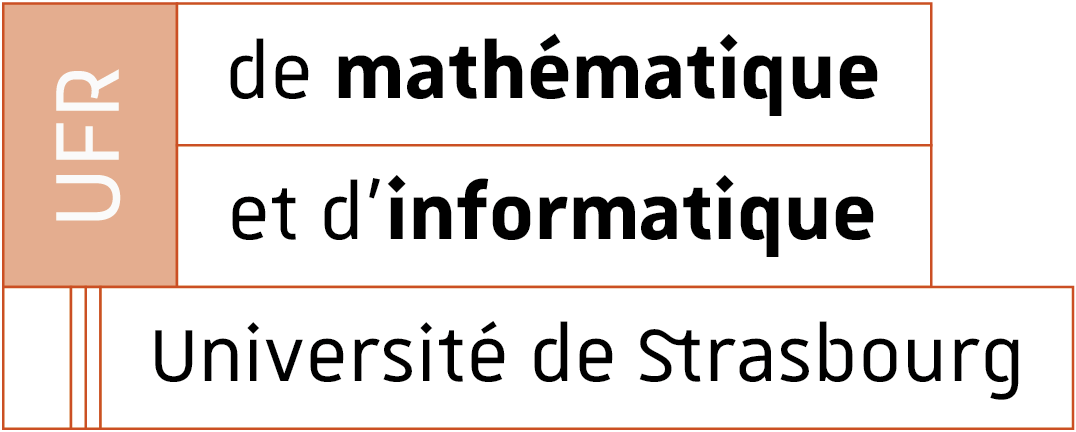
\includegraphics[width=0.25\textwidth]{images/logo-ufr.png} \hspace{1cm}
    
\includegraphics[width=0.25\textwidth]{images/logo-cemosis.png} \hspace{1cm}
    
\includegraphics[width=0.25\textwidth]{images/logo-numpex.png} \\
    \vspace{1cm} % Adjust space between rows
    
\includegraphics[width=0.25\textwidth]{images/logo-irma.png} \hspace{1cm}
    
\includegraphics[width=0.25\textwidth]{images/logo-inria.png} \hspace{1cm}
    
\includegraphics[width=0.25\textwidth]{images/logo-hidalgo2.png} \\
\end{figure}

\vspace{2cm}
{\huge\bfseries Exa-MA WP1 - Vegetation\par}
\vspace{1cm}
{\Large\itshape Internship report\par}
{\Large Pierre-Antoine SENGER\par}
\vspace{1cm}
supervised by\par
Vincent CHABANNES\par

\vfill

% Bottom of the page
{\large Date: \today\par}
\end{titlepage}

\tableofcontents

\newpage

\section{Introduction}

This project is part of a group of projects conducted within the \texttt{Exa-MA Project}
\cite{exaMA} which is a part of the \texttt{Numpex} project research\cite{numpex}. 
Those are the different projects my colleagues and I worked on:
\begin{itemize}
    \item \texttt{Exa-MA WP1 - Vegetation}
    \item \texttt{Exa-MA WP1 - Terrain}
    \item \texttt{Exa-MA WP1 - Urban Building LOD-1}
    \item \texttt{Exa-MA WP1 - Urban Building LOD-2 and Kinetic}
    \item \texttt{Exa-MA WP1 - Performance and Scalability}
\end{itemize}

These projects are conducted within the \texttt{HiDALGO2}\cite{hidalgo2} initiative, which
"aims to explore synergies between modeling, data acquisition, simulation,
data analysis and visualization along with achieving better scalability on
current and future HPC and AI infrastructures to deliver highly-scalable
solutions that can effectively utilize pre-exascale systems."\cite{hidalgo2-about}

Specifically focusing on the \texttt{Urban Building Model}\cite{hidalgo2-ubm}
Use Case (UBM) which is "developing the Urban Building pilot application to
improve building energy efficiency and indoor air quality"\cite{hidalgo2-ubm},
this particular project aims to integrate vegetation, particularly trees, into 3D models
of urban environments.

The projects are conducted within \texttt{Cemosis}\cite{cemosis} (Center for
Modeling and Simulation in Strasbourg), which is hosted by
\texttt{IRMA}\cite{irma} (Institute for Advanced Mathematical Research) at
\texttt{Strasbourg University}. We operated as students under the supervision of
 \texttt{Vincent Chabannes}\cite{chabannes}, research engineer at IRMA and 
 \texttt{Christophe Prud'homme}\cite{prudhomme}, professor in applied mathematics
  at Strasbourg University.

\subsection{Context}

Urban areas are complex ecosystems influenced by various factors, with
vegetation, especially trees, playing a crucial role in shaping microclimates,
reducing energy consumption, and enhancing overall livability\cite{TIR4sTREEt}.

\begin{figure}[H]
    \begin{minipage}{0.45\textwidth}
        \centering
        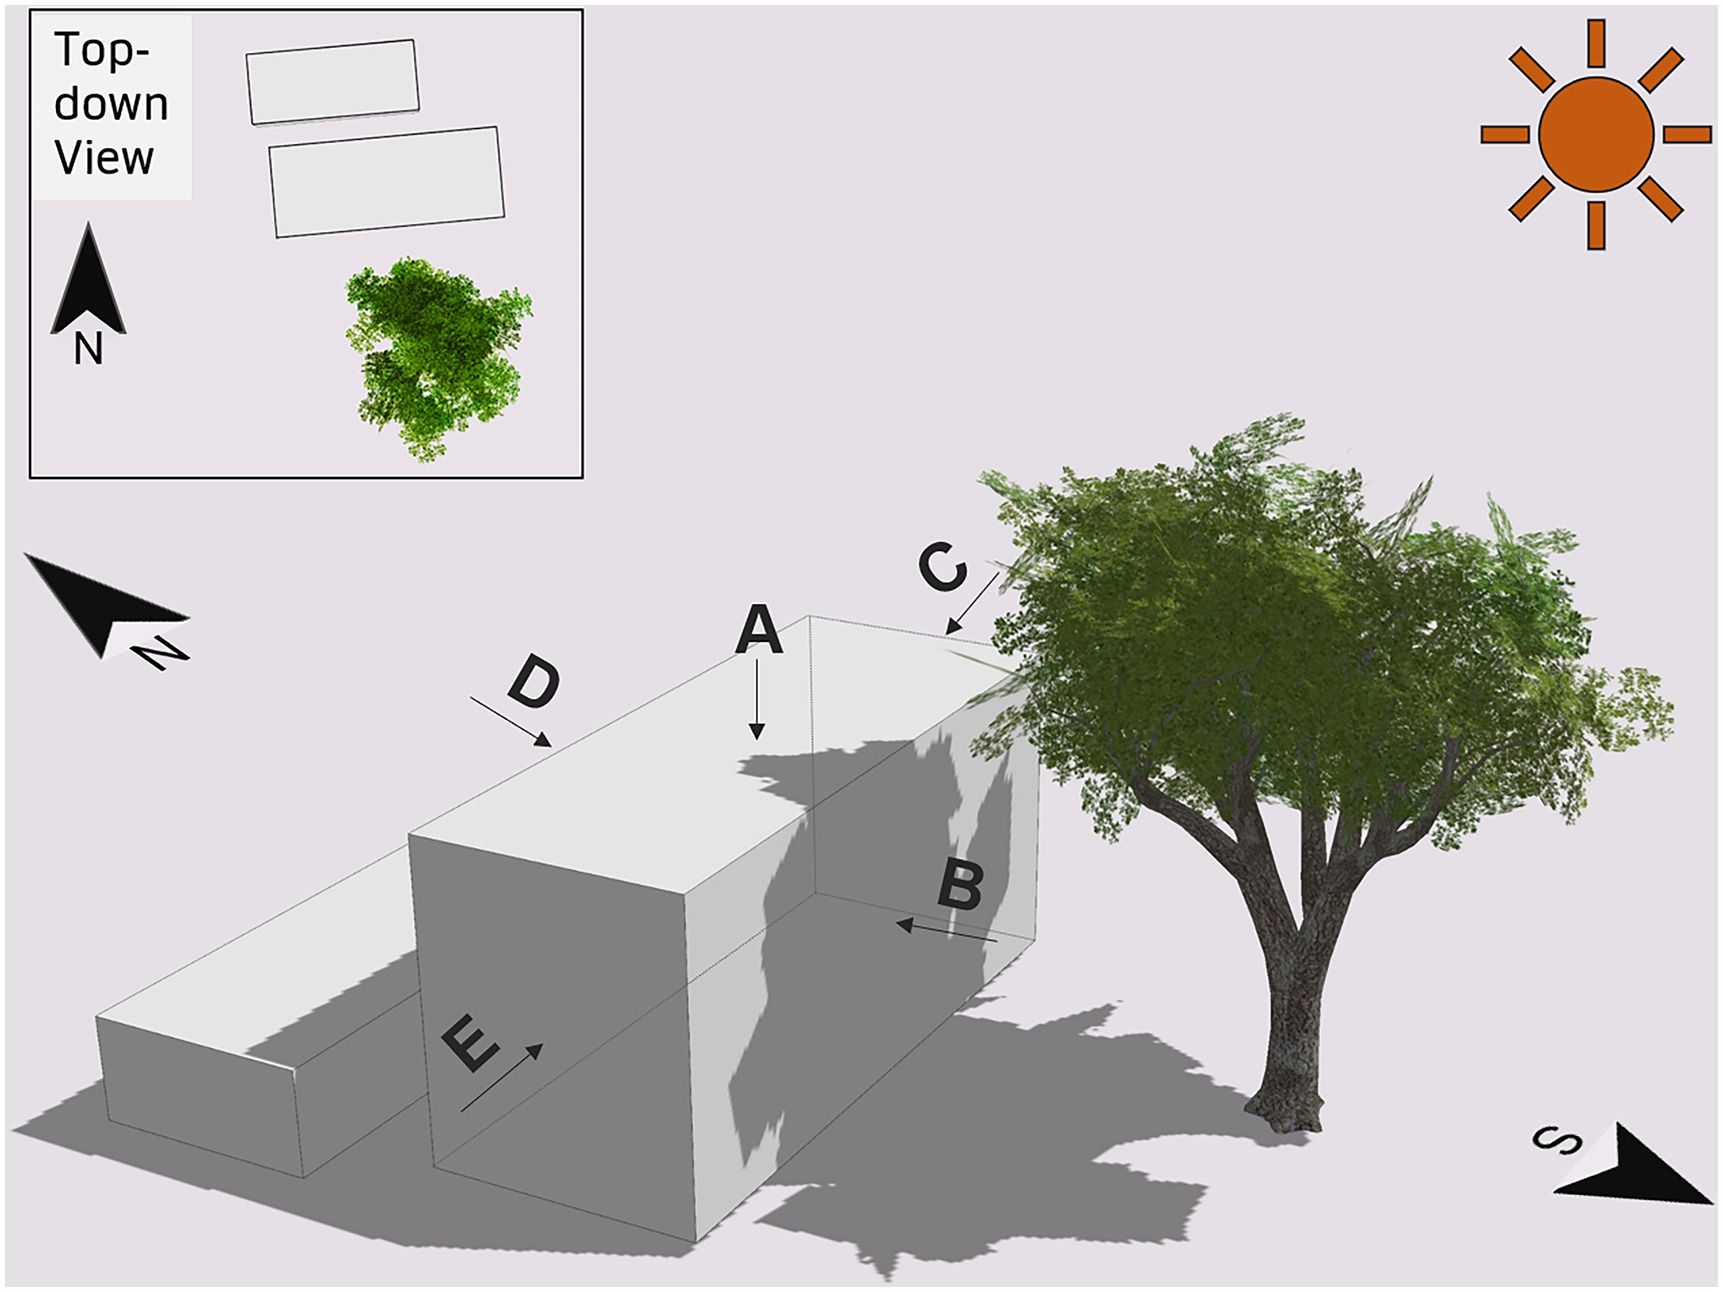
\includegraphics[width=1\textwidth]{images/tree-shade.png}
        \captionsetup{font={scriptsize}}
        \caption{Tree providing shade to a building \cite{img:TreeShade}}
    \end{minipage}
    \begin{minipage}{0.45\textwidth}
        \centering
        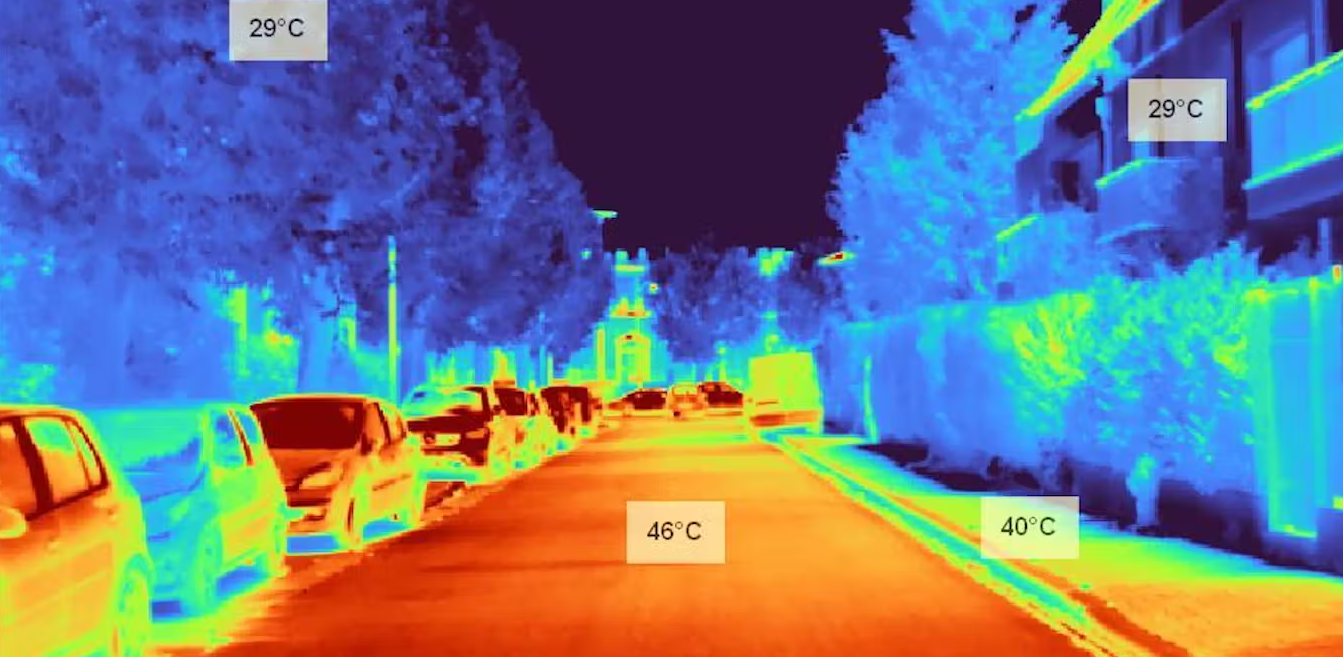
\includegraphics[width=1\textwidth]{images/heat-street.png}
        \captionsetup{font={scriptsize}}
        \caption{Thermal image of a street depicting heat distribution \cite{img:street_thermography}}
    \end{minipage}
\end{figure}

This \texttt{Vegetation} project aims to integrate trees into 3D geometric models of urban
environments to improve the accuracy and realism of thermal and energy
simulations.

By leveraging data from \texttt{OpenStreetMap}\cite{openstreetmap}, a
collaborative free geographic database, we will use \texttt{CGAL}\cite{cgal},
an open source software library of computational geometry algorithms, and
\texttt{Gmsh}\cite{gmsh}, a 3D finite element mesh generator,
to generate 3D tree models and integrate them into terrain meshes.

Our primary focus will be on Strasbourg, France. More specifically, we were
provided with an \texttt{.stl}\cite{stl} file containing a 3D model of the
Strasbourg city center:

\begin{figure}[H]
    \centering
    \begin{minipage}{0.45\textwidth}
      \centering
      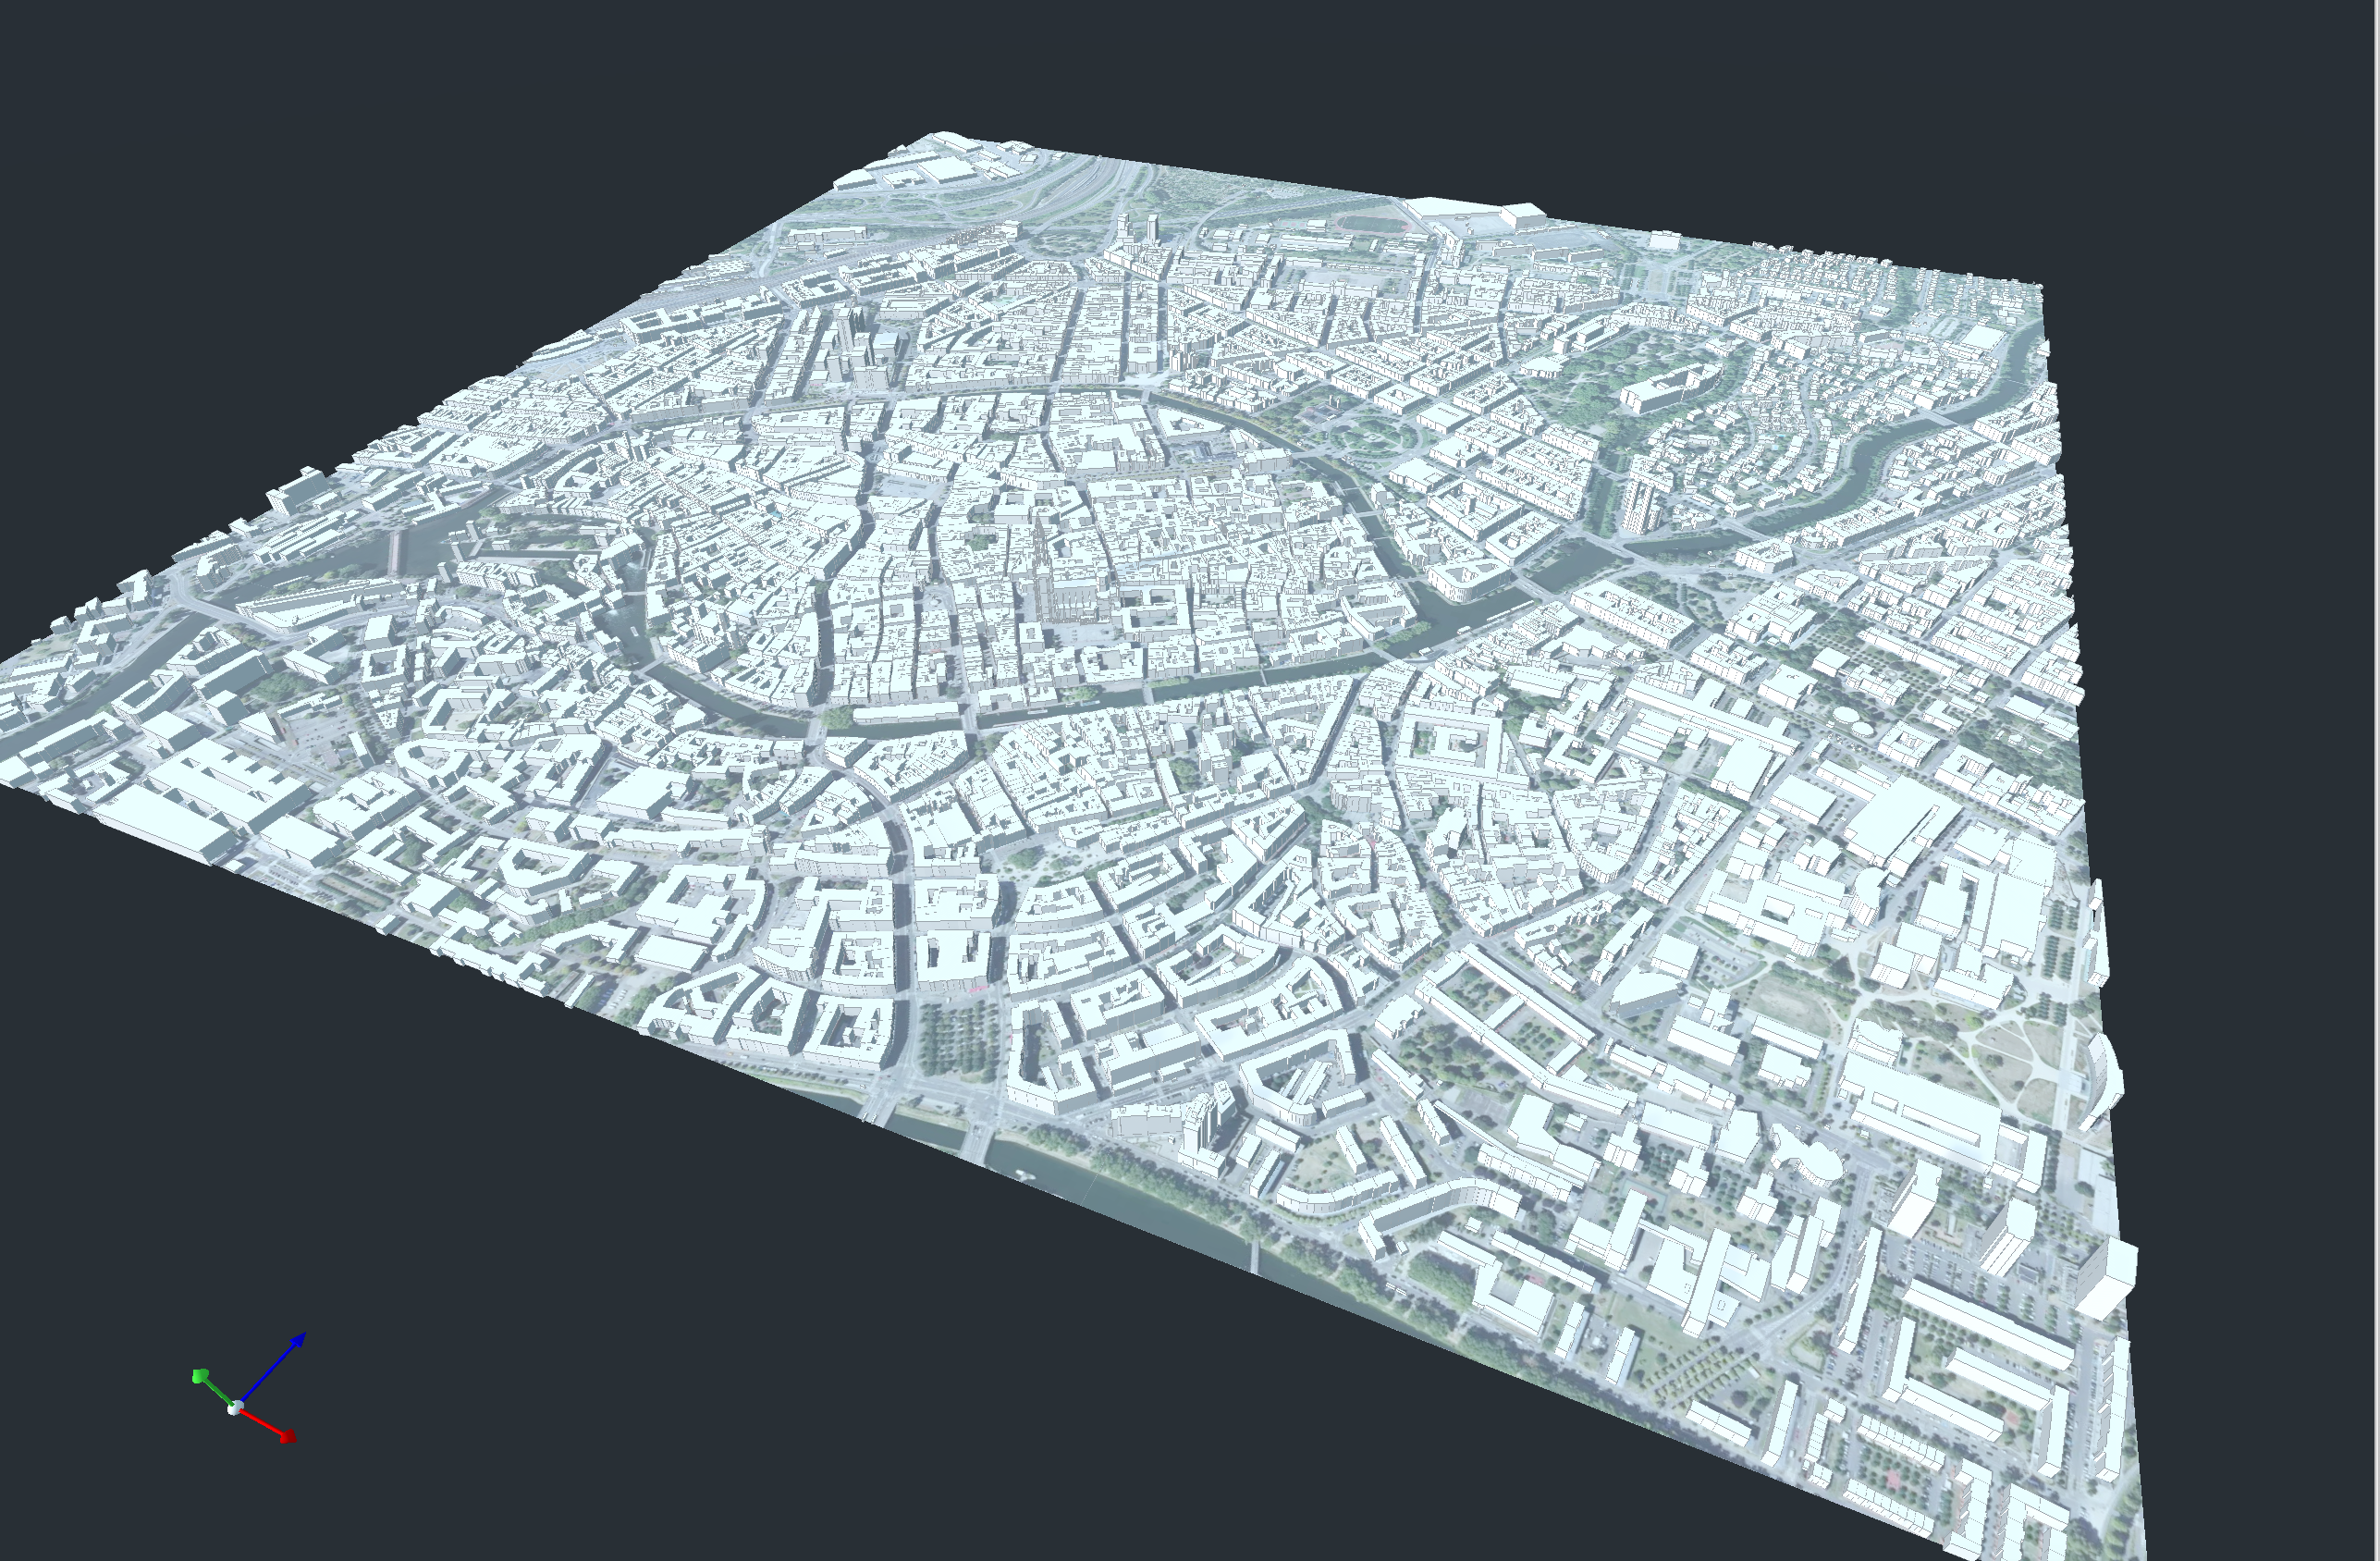
\includegraphics[width=1\textwidth]{images/strasbourg-mesh-1.png}
      \captionsetup{font={scriptsize}}
      \caption{Strasbourg 3D model (1)}
    \end{minipage}
    \begin{minipage}{0.45\textwidth}
      \centering
      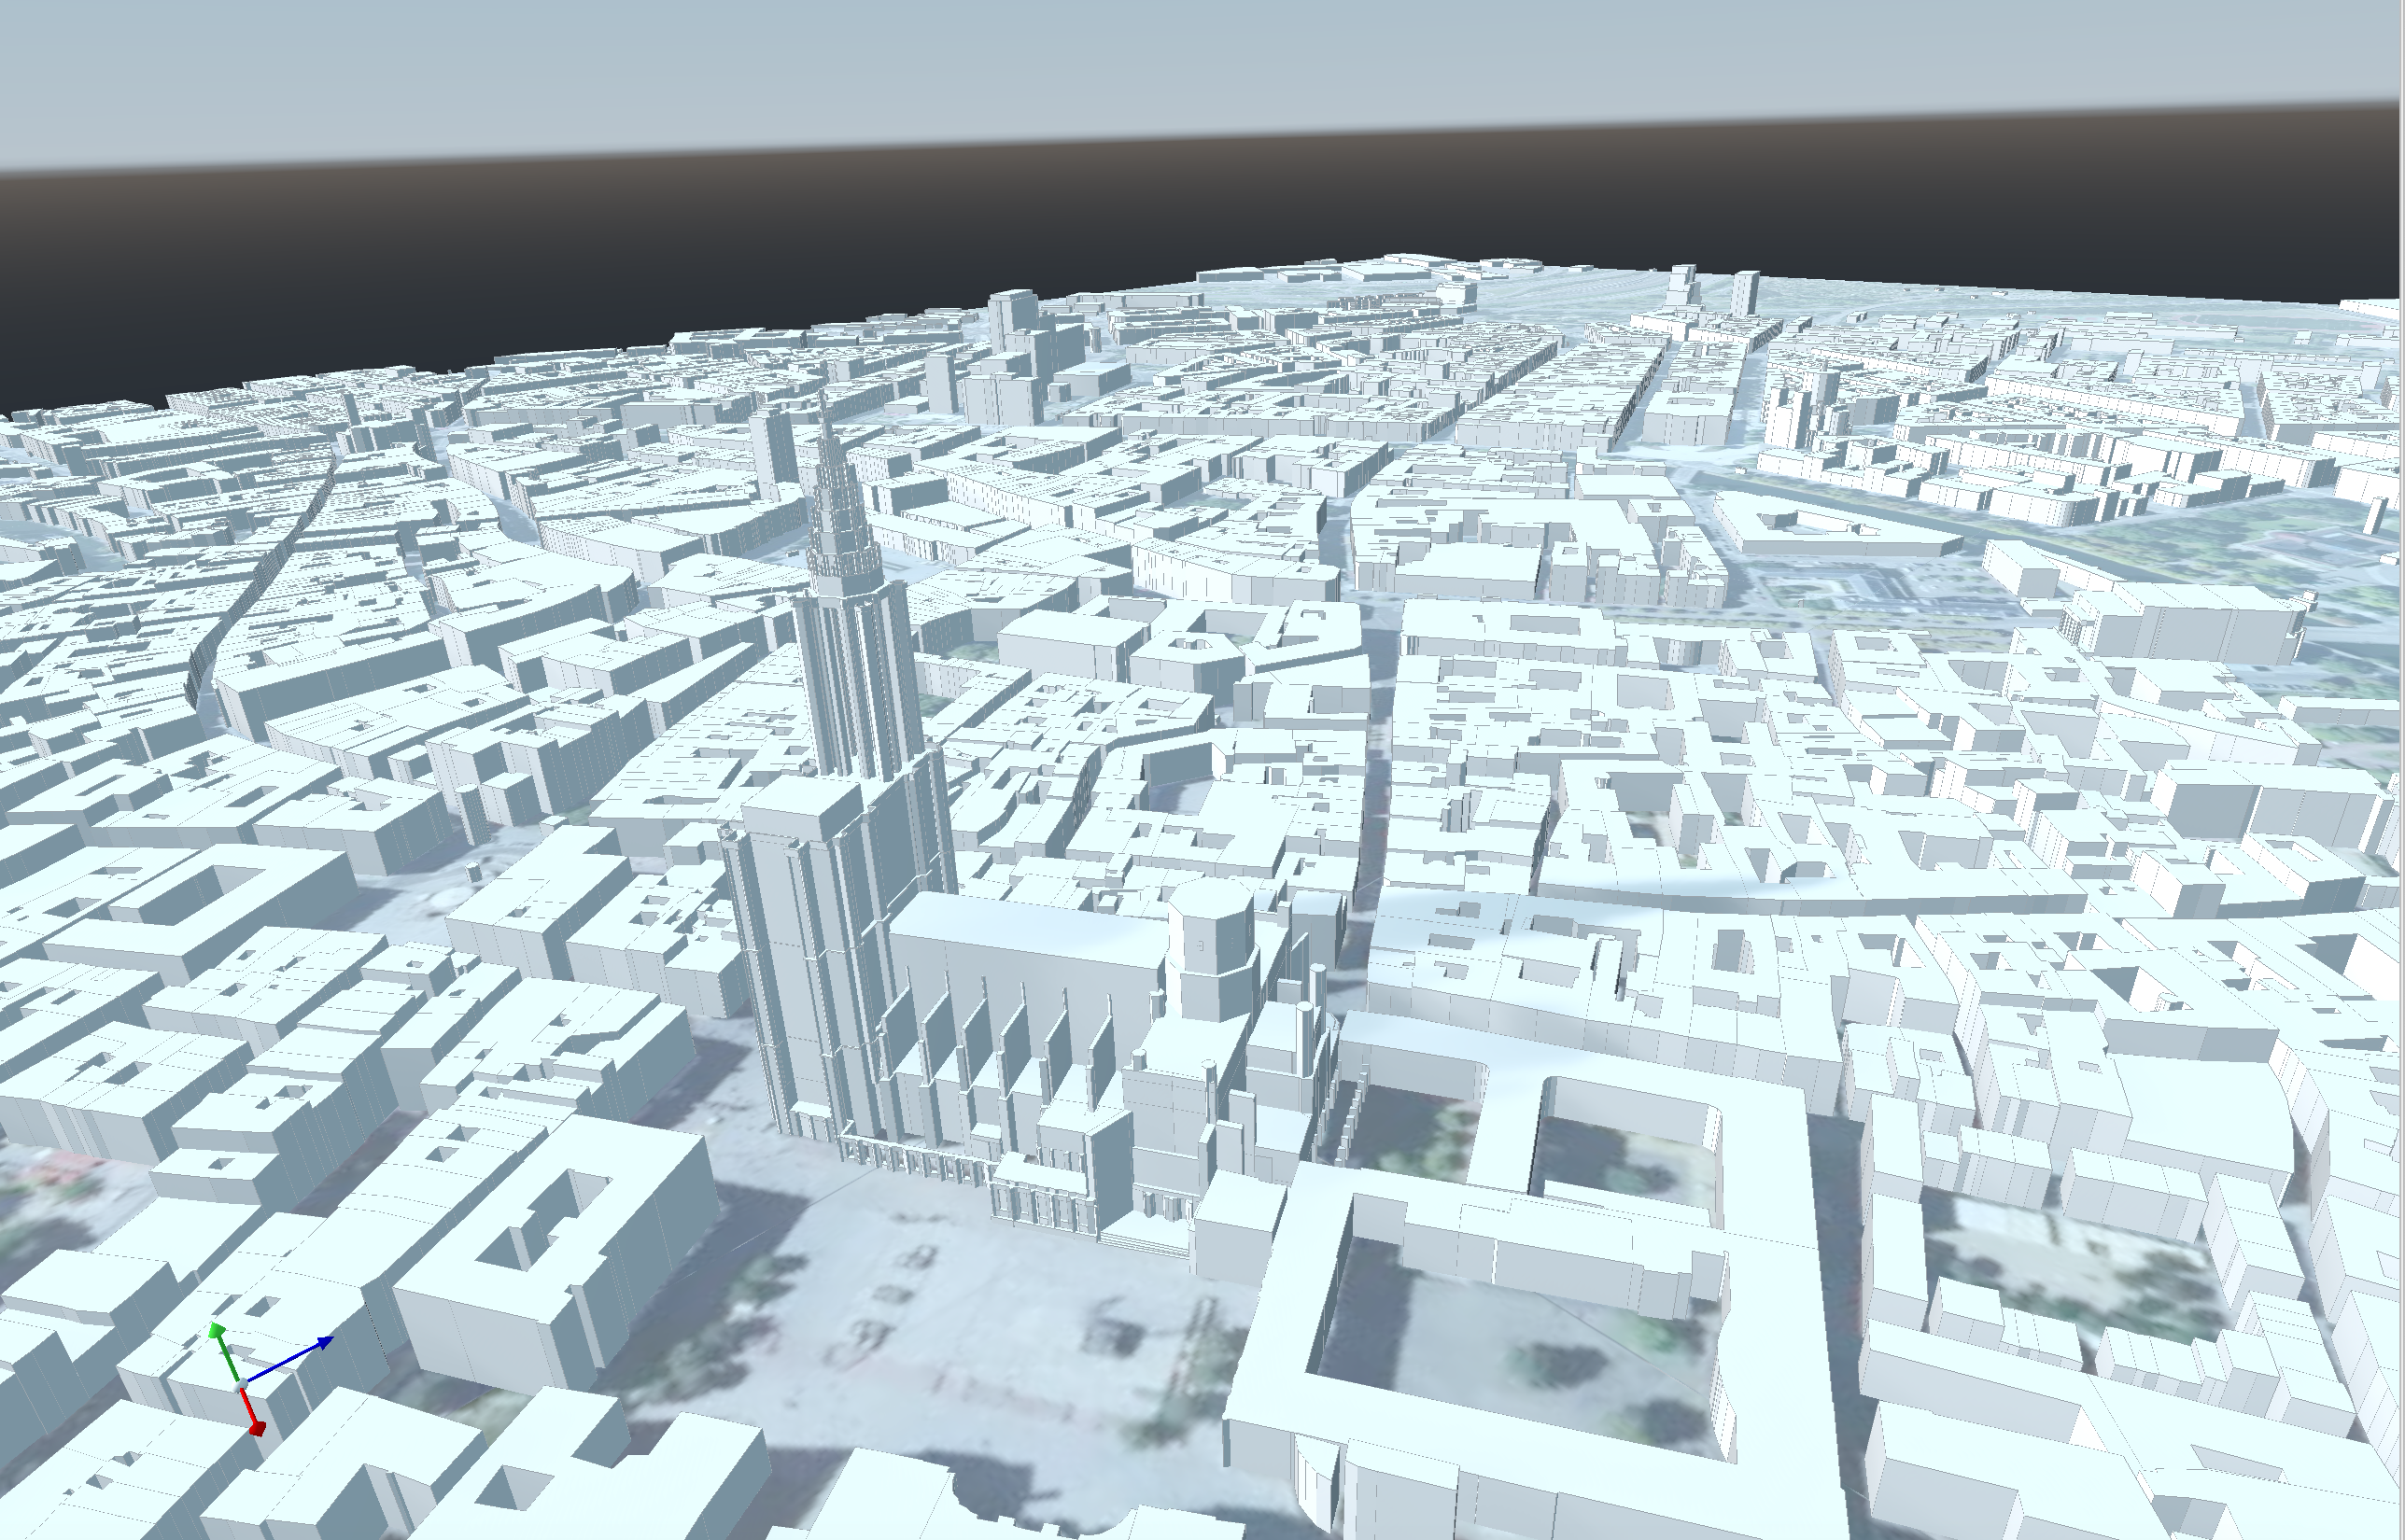
\includegraphics[width=1\textwidth]{images/strasbourg-mesh-2.png}
      \captionsetup{font={scriptsize}}
      \caption{Strasbourg 3D model (2)}
    \end{minipage}
\end{figure}

However, the final version of the software will be designed to be easily adaptable to any area.
Here's an example of a 3D model of Manhattan, NYC:

\begin{figure}[H]
    \centering
    \begin{minipage}{0.45\textwidth}
      \centering
      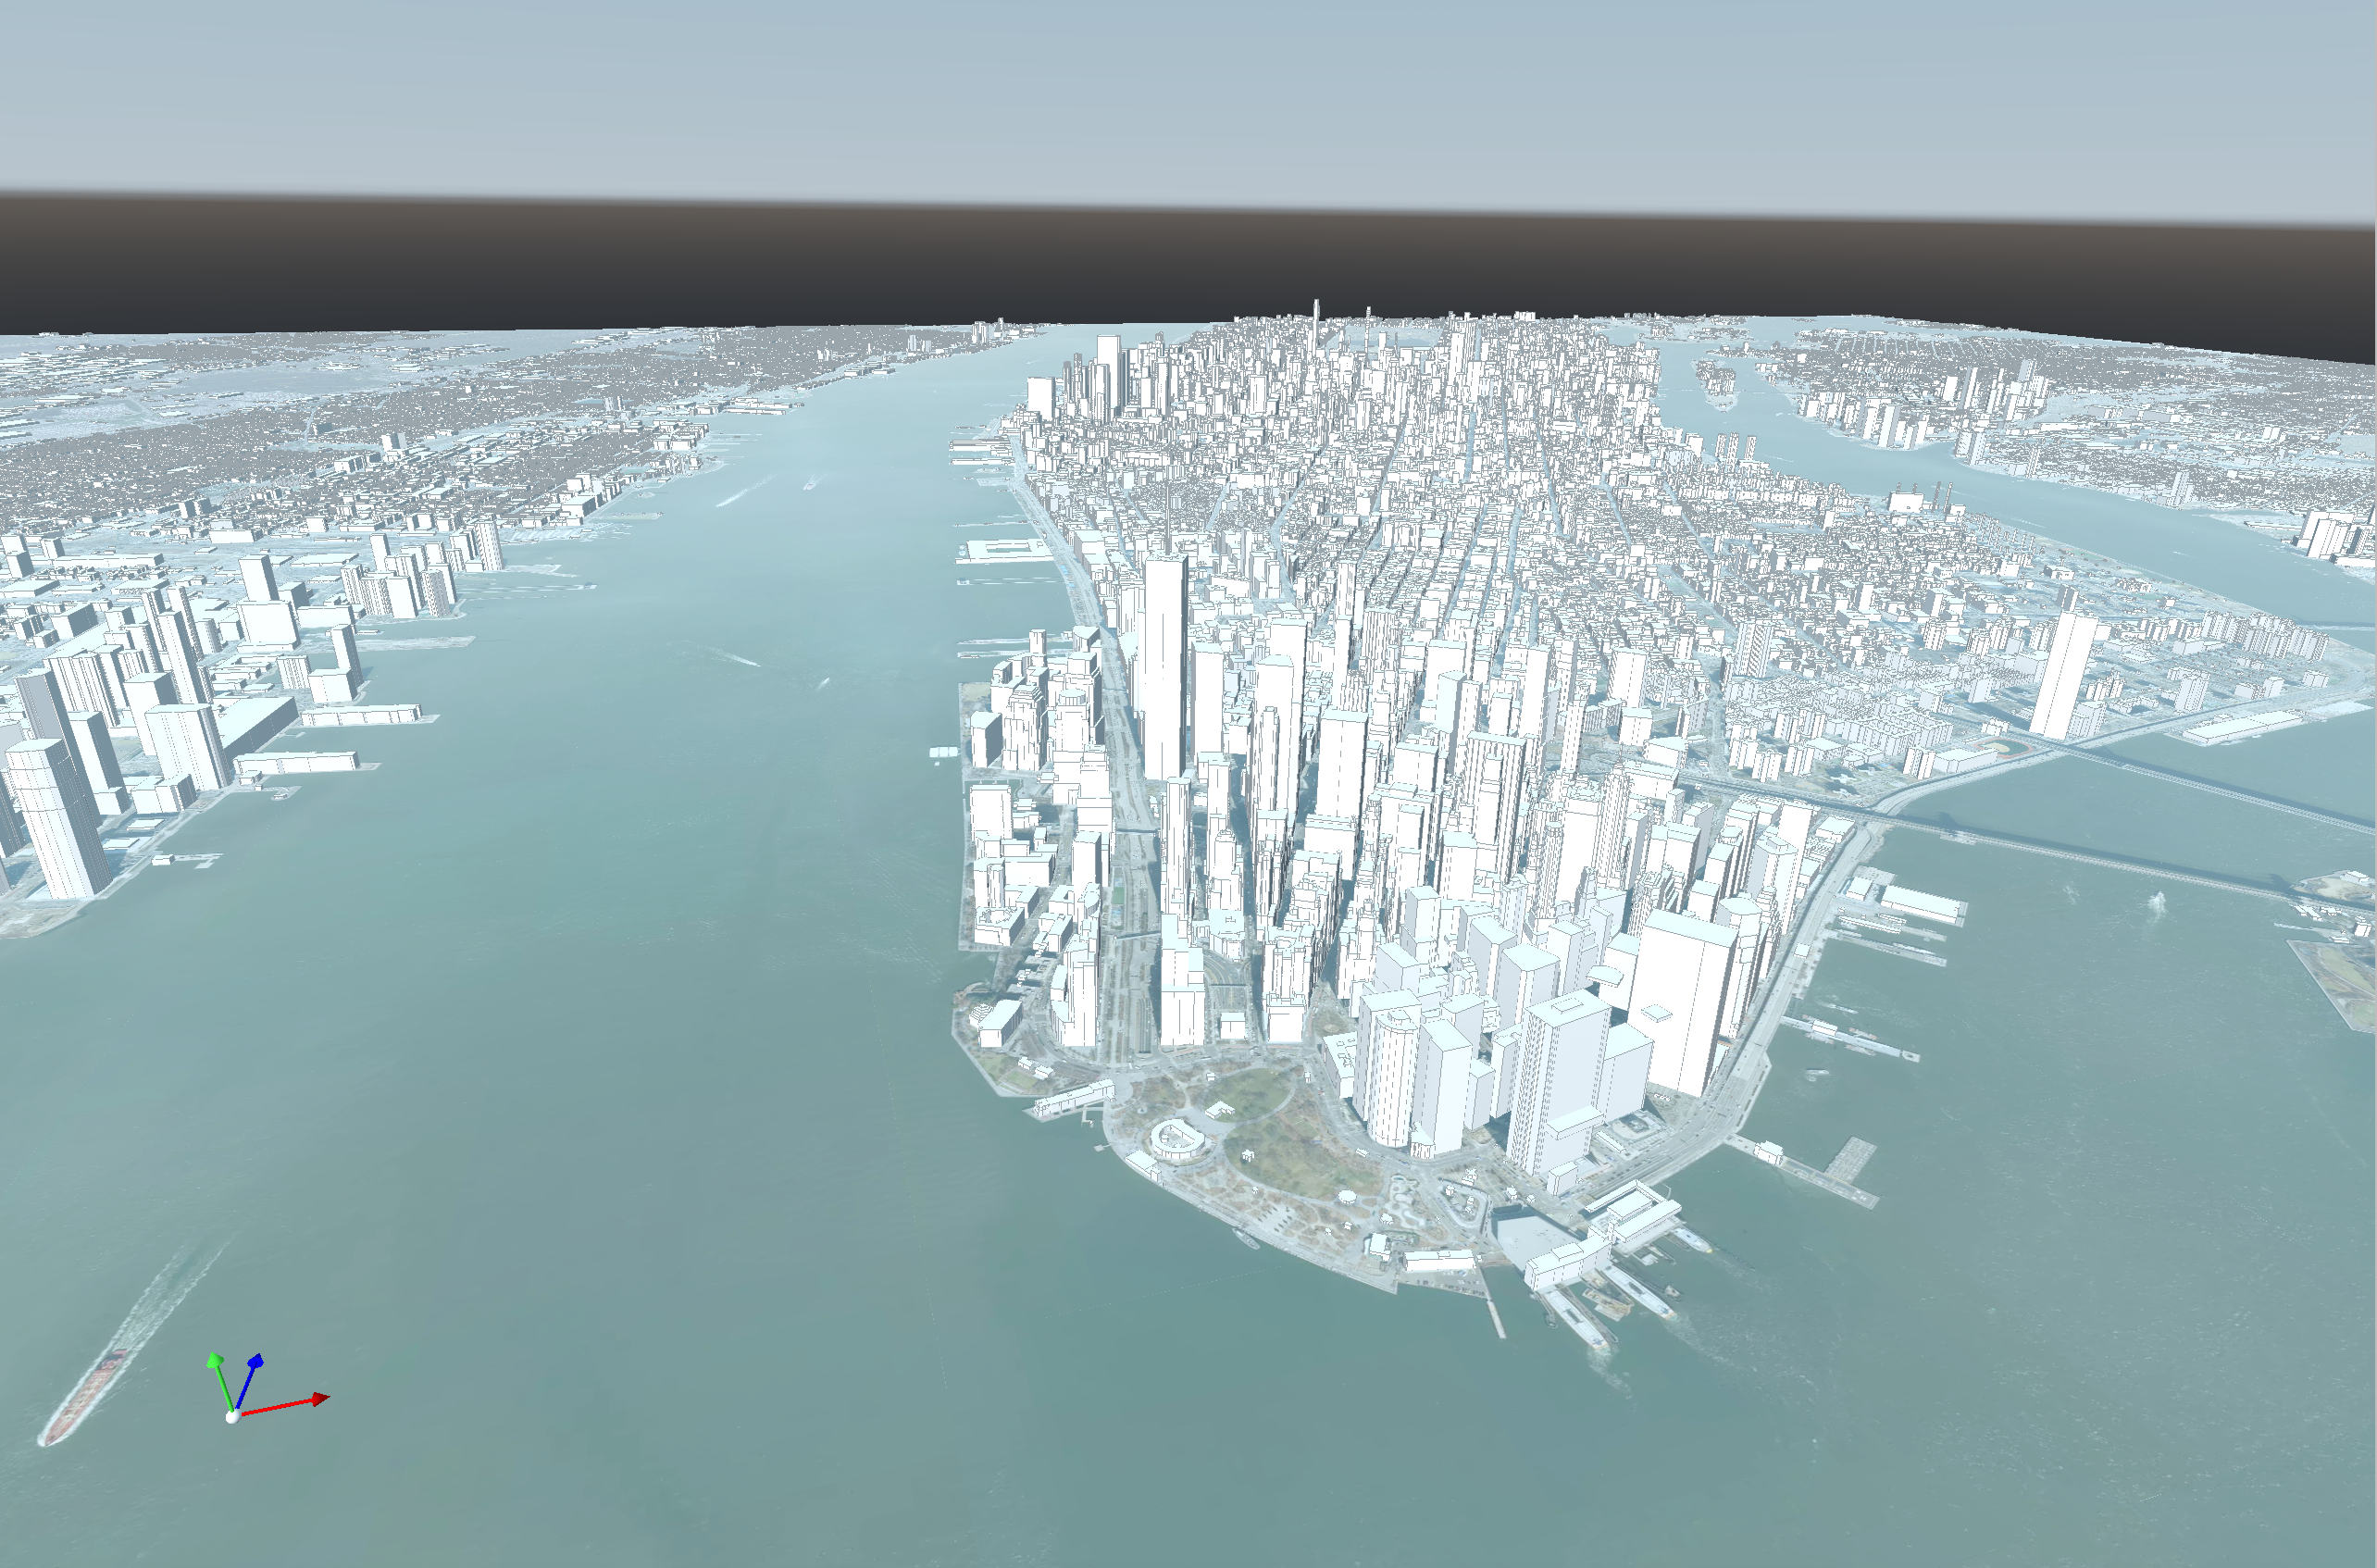
\includegraphics[width=1\textwidth]{images/mesh-manhattan-1.png}
      \captionsetup{font={scriptsize}}
      \caption{Manhattan 3D model (1)}
    \end{minipage}
    \begin{minipage}{0.45\textwidth}
      \centering
      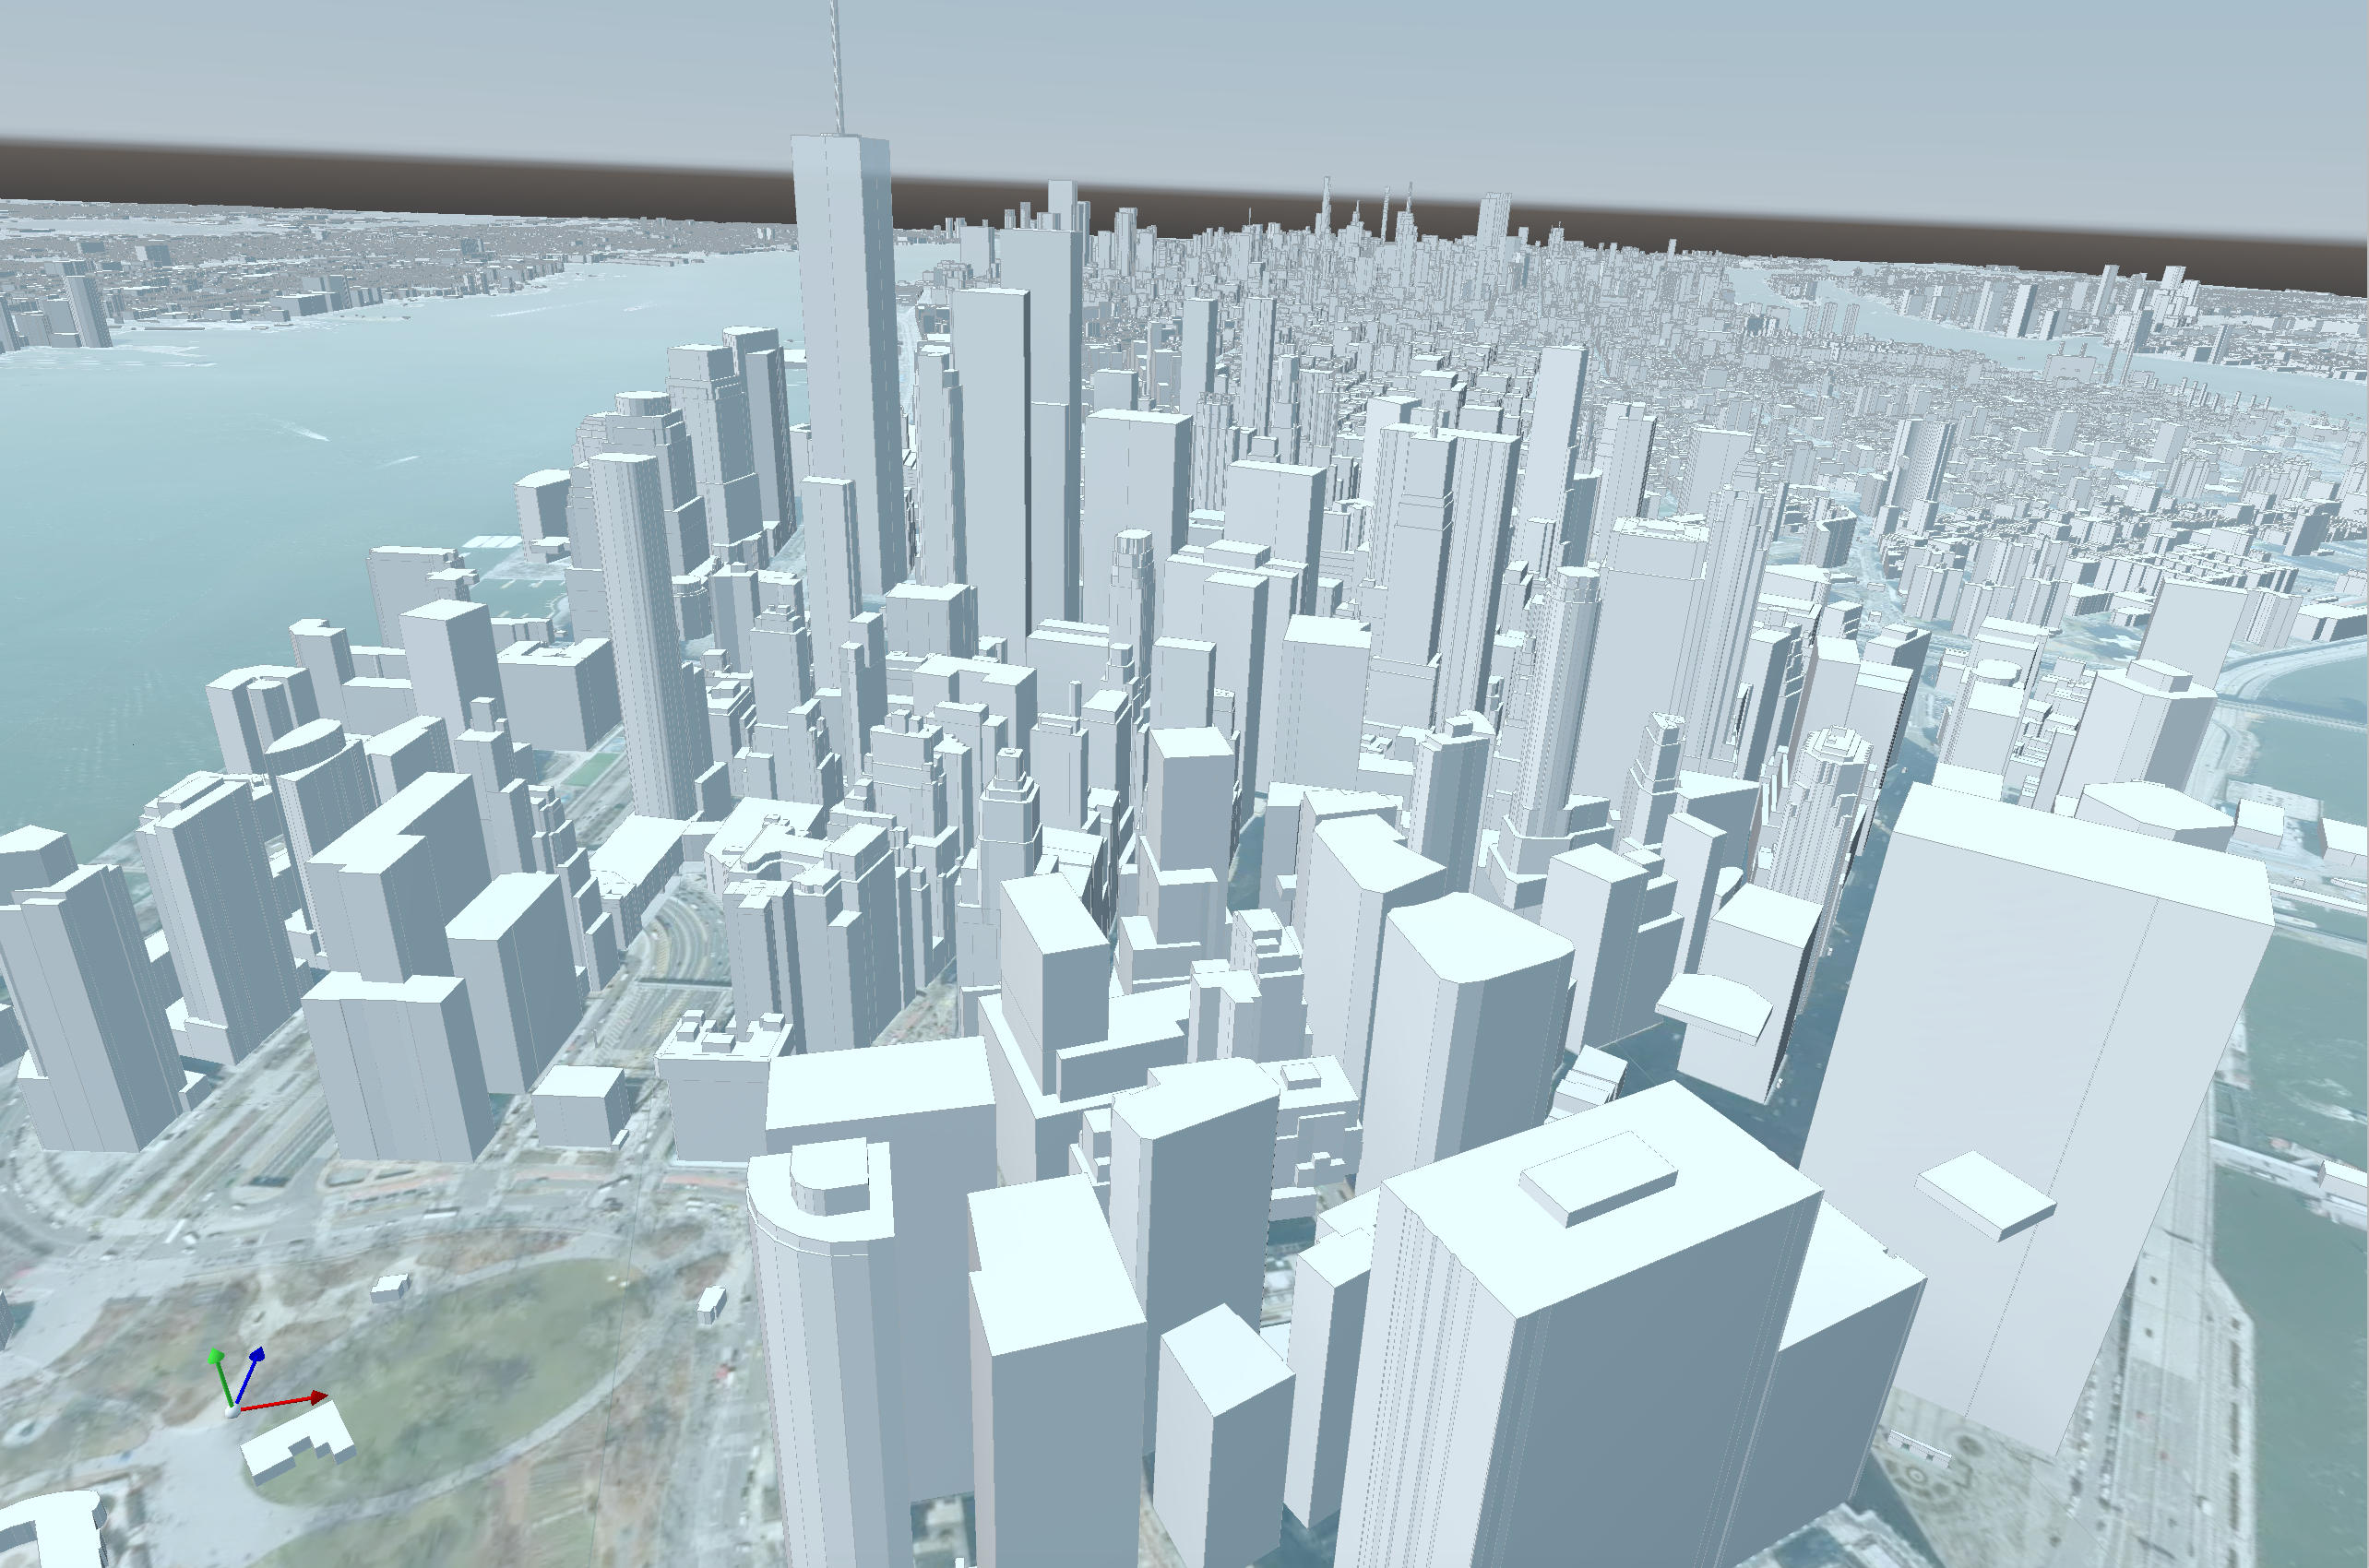
\includegraphics[width=1\textwidth]{images/mesh-manhattan-2.png}
      \captionsetup{font={scriptsize}}
      \caption{Manhattan 3D model (2)}
    \end{minipage}
\end{figure}

\subsection{Main objectives}

\begin{itemize}
    \item Extracting tree meta-data from \texttt{OpenStreetMap} using \texttt{cpr}\cite{cpr}.
    \subitem Position (latitude, longitude). In a park, boarding a road, etc.
    \subitem Height, genus, species, crown diameter, circumference, etc.
    \item Generating 3D tree models using \texttt{CGAL}\cite{cgal} and \texttt{Gmsh}\cite{gmsh}.
    \subitem LOD 0, 1, 2, 3.
    \subitem Different leaf density.
    \item Integrating tree models into the terrain mesh we already have.
    \subitem Avoiding collision between trees and buildings.
    \subitem Taking into account terrain elevation.
    \item Optimizing and parallelizing the algorithms to efficiently handle large datasets.
\end{itemize}

\subsection{Software and libraries}
To source our data, we'll utilize the \texttt{Overpass API}\cite{overpass} a
read-only API to query data from \texttt{OpenStreetMap}, alongside
 \texttt{cpr}\cite{cpr} (a wrapper around \texttt{cURL}\cite{curl}), a URL transfer library. For geometric modeling, we
will utilize the \texttt{Gmsh}\cite{gmsh} library as well as the \textbf{master}
 \texttt{CGAL} library, available on
GitHub\cite{cgal-master}, known for its efficiency and reliability in geometric
computation.

\subsection{GitHub repository}
We created a \href{https://github.com/feelpp/ktirio-geom}{GitHub}
repository to manage the project and facilitate collaboration.
The repository contains the project's code, documentation, and resources.
It will be updated regularly to reflect the progress and changes made during
the project's development.


\section{Methodology}

\subsection{Data acquisition}

We will use the \texttt{Overpass API} and \texttt{cpr} to query
\texttt{OpenStreetMap} for all the available tree data within the specified
bounding box:

\begin{lstlisting}[language=C++]
std::string query =
    "[out:json]; (node(" + bbox + ")[\"natural\"=\"tree\"];); out;";
    std::cout << "Query: " << query << std::endl;

cpr::Response r = cpr::Post(
    cpr::Url{"http://overpass-api.de/api/interpreter"}, cpr::Body{query},
    cpr::Header{{"Content-Type", "application/x-www-form-urlencoded"}},
    cpr::Timeout{10000} // Set a timeout of 10 seconds
);
\end{lstlisting}

The \texttt{http://overpass-api.de/api/interpreter} endpoint interprets and
executes the \texttt{Overpass QL}\cite{overpass-ql} queries, retrieving
specific parts of the \texttt{OpenStreetMap} data. In this case, the query
fetches all nodes within the given bounding box tagged as \texttt{natural=tree}.

If the query is not successful, a \texttt{cpr.log} file will be generated to
store the error message. Otherwise, the data will be stored in a \texttt{.json}.

A \textit{config.json} file is available for the user to specify the area of
interest and other parameters:

\begin{lstlisting}[language=json]
{
    "bbox": "48.5750,7.7394,48.5919,7.7621",
    "origin": "48.583055227464364, 7.748664426560083",
    "LOD": 3,
    "default_height_range": "3, 6",
    "input_building_mesh": "mesh_lod1.stl",
    "merge_buildings_trees": true,
    "output_name": "grande_ile"
}
\end{lstlisting}

Where :
\begin{itemize}
    \item \texttt{bbox}: is the bounding box for the query in the format:
    \subitem (SW latitude, SW longitude, NE latitude, NE longitude)
    \item \texttt{origin}: is the origin of the 3D space in latitude and longitude
    used to convert the GPS coordinates to Cartesian coordinates. It must be the
    same for the terrain mesh and the tree meshes.
    \item \texttt{LOD}: is the level of details of the meshes (0, 1, 2 or 3)
    \item \texttt{default\_height\_range}: is a range used to randomly assign a
    height to trees that do not have one.
    \item \texttt{input\_building\_mesh}: is the name of the input file
    representing the terrain mesh.
    \item \texttt{merge\_buildings\_trees}: is a boolean indicating whether the
    buildings and trees should be merged into a single mesh or not.
    \item \texttt{output\_name}: is the base name of the output file
    representing the unions of the tree meshes.
\end{itemize}

The data will be stored in \textit{query\_result.json} file in the root directory
 of the project. \\
Here is an example of the query result for one tree:

\begin{lstlisting}[language=json]
{
    "type": "node",
    "id": 10162018740,
    "lat": 48.5850910,
    "lon": 7.7502624,
    "tags": {
        "circumference": "1.47655",
        "diameter_crown": "5",
        "genus": "Platanus",
        "height": "6",
        "leaf_cycle": "deciduous",
        "leaf_type": "broadleaved",
        "natural": "tree",
        "ref": "16401",
        "source": "data.strasbourg.eu - patrimoine_arbore",
        "source:date": "2022-01-02",
        "species": "Platanus acerifolia x",
        "species:wikidata": "Q24853030"
    }
}
\end{lstlisting}

Sometimes, multiple \texttt{tags} are missing, as shown here:

\begin{lstlisting}[language=json]
{
    "type": "node",
    "id": 4439566691,
    "lat": 48.5839128,
    "lon": 7.7487125,
    "tags": {
      "natural": "tree"
    }
}
\end{lstlisting}

We will primarily use the \texttt{position} of the tree (latitude and
longitude), its \texttt{height}, \texttt{circumference} and \texttt{diameter\_crown}.

\subsection{Tree library}
We will assume that the trees belongs to a specific shape category (cone, oval, 
round). This could be improved by adding more shape as shown in the next image:
\begin{figure}[H]
    \centering
    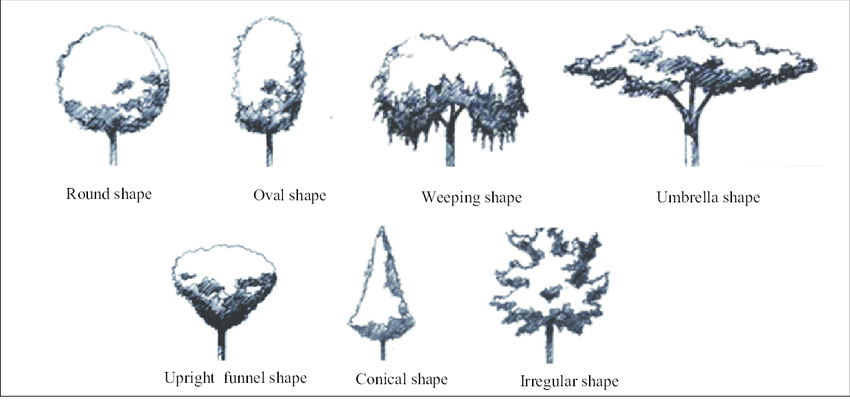
\includegraphics[width=0.8\textwidth]{images/Different-types-of-the-trees-shape.png}
    \captionsetup{font={scriptsize}}
    \caption{Different tree shapes\cite{img:tree-shape}}
\end{figure}


For all tree LODs we will separate the tree into two parts: the trunk and the
foliage. The trunk will be a simple cylinder, while the foliage will be a more 
complex geometry. This will allow us to treat the foliage separately which will 
be useful for scaling and when considering different leaf densities.

\subsubsection{LOD 0}
For the lowest level of detail, we will use simple models manually made with 
\texttt{Gmsh}\cite{gmsh} and store them in \texttt{data/vegetation/tree\_ref} 
(the \texttt{Gmsh} source code is available in \texttt{data/vegetation/tree\_ref/tree\_ref\_geo}). 
In the following images, we can see the trunk and foliage of the tree, with the 
trunk separated from the foliage:

\begin{figure}[H]
    \centering
    \begin{minipage}{0.45\textwidth}
        \centering
        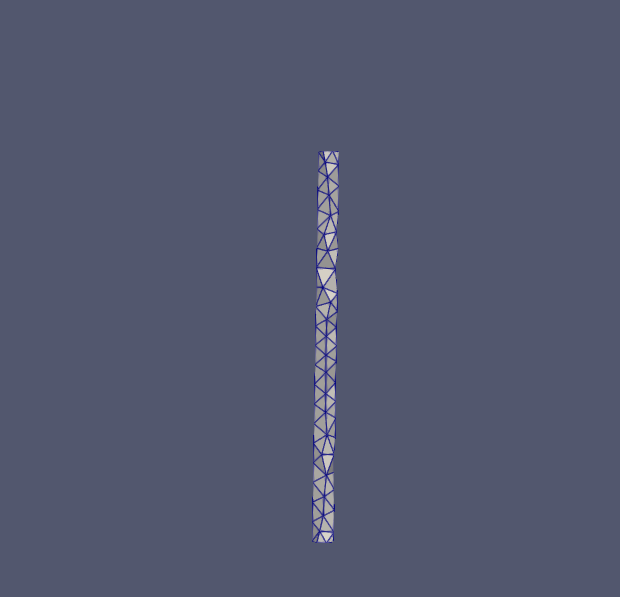
\includegraphics[width=1\textwidth]{images/tree-trunk.png}
        \captionsetup{font={scriptsize}}
        \caption{Tree trunk}
    \end{minipage}
    \begin{minipage}{0.45\textwidth}
        \centering
        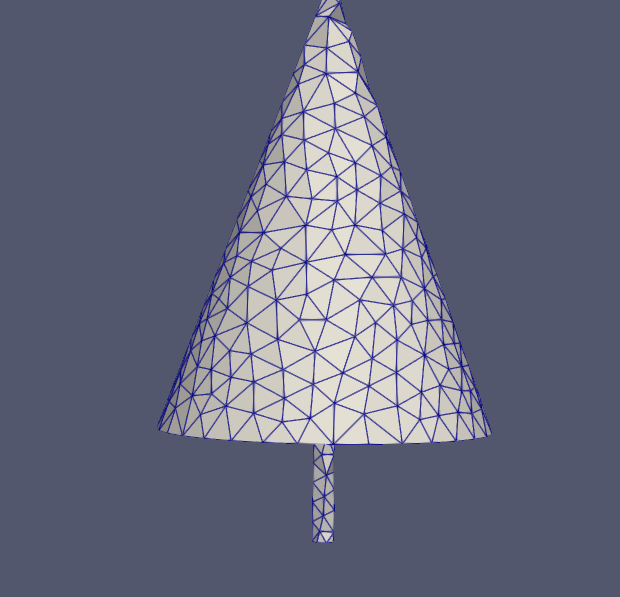
\includegraphics[width=1\textwidth]{images/tree-cone_lod0.png}
        \captionsetup{font={scriptsize}}
        \caption{Cone shaped tree lod0}
    \end{minipage}
\end{figure}

\begin{figure}[H]
    \centering
    \begin{minipage}{0.45\textwidth}
        \centering
        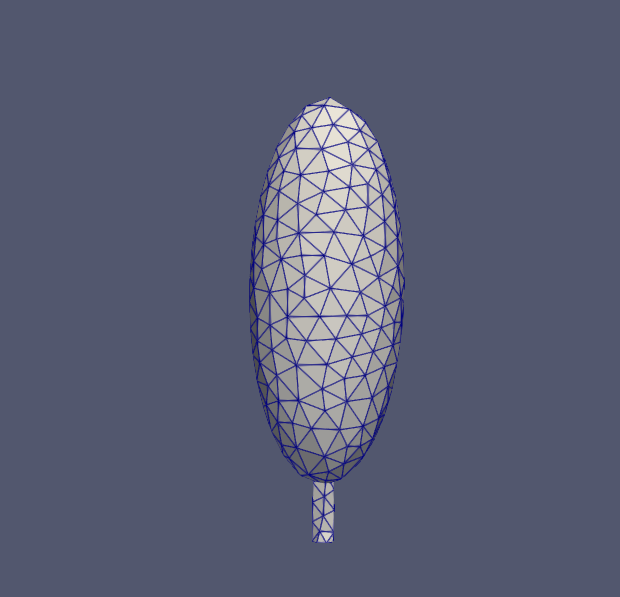
\includegraphics[width=1\textwidth]{images/tree-oval_lod0.png}
        \captionsetup{font={scriptsize}}
        \caption{Oval shaped tree lod0}
    \end{minipage}
    \begin{minipage}{0.45\textwidth}
        \centering
        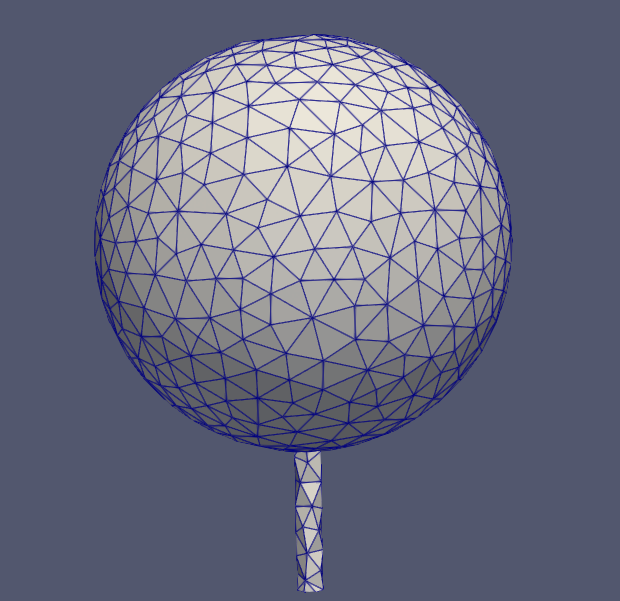
\includegraphics[width=1\textwidth]{images/tree-round_lod0.png}
        \captionsetup{font={scriptsize}}
        \caption{Round shaped tree lod0}
    \end{minipage}
\end{figure}

\subsubsection{LOD 1, 2, 3}
As for the other LODs, we will retrieve reference trees meshes from the
\texttt{Sketch up 3D Warehouse}\cite{sketchup} as shown in the next image:
\begin{figure}[H]
    \centering
        \centering
        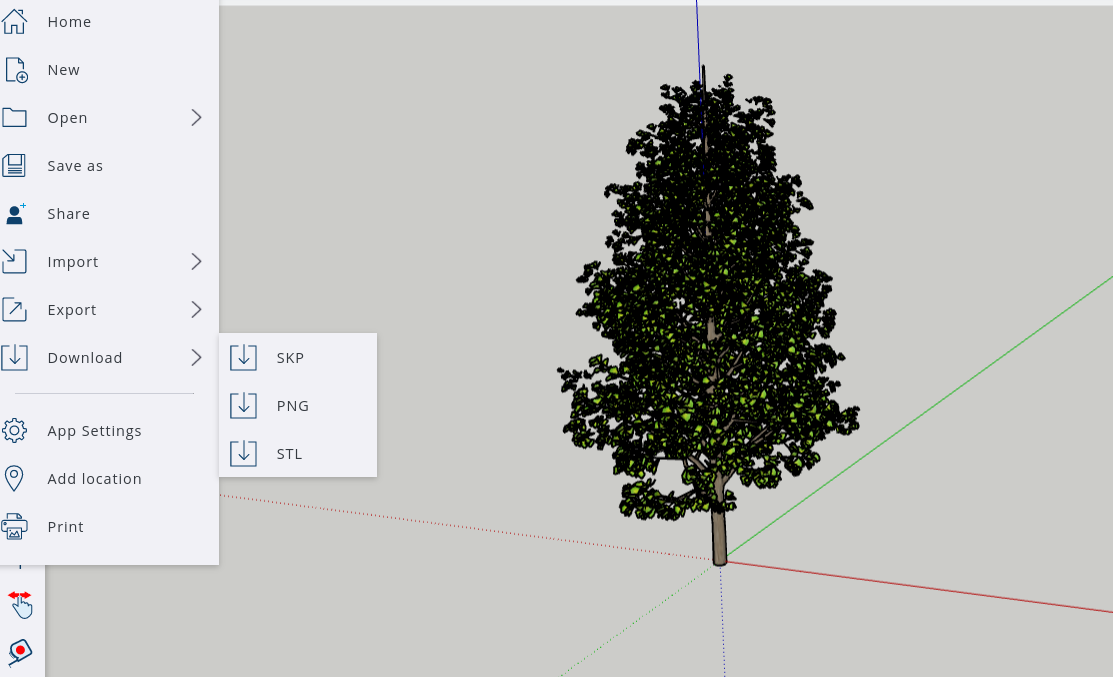
\includegraphics[width=0.8\textwidth]{images/ginkgo-sketchup.png}
        \captionsetup{font={scriptsize}}
        \caption{Mesh of a Ginkgo tree on Sketchup 3D Warehouse}
\end{figure}

We will then preprocess these models using \texttt{Meshlab}\cite{meshlab}, removing 
the trunk and branches as much as possible. Additionally, we will normalize them
 to fit within a unit bounding box and translate them to the origin. These cleaned
  models will be stored in the \texttt{data/vegetation/tree\_ref/tree\_ref\_sketchup} directory.
 The results are as follows:

\begin{figure}[H]
    \centering
    \begin{minipage}{0.30\textwidth}
        \centering
        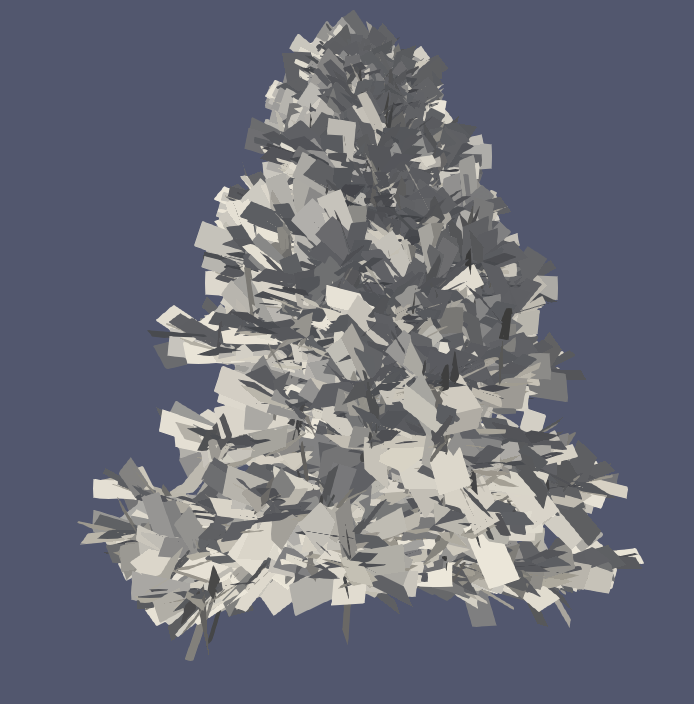
\includegraphics[width=1\textwidth]{images/tree-conifer.png}
        \captionsetup{font={scriptsize}}
        \caption{A cleaned conifer (Cone tree)}
    \end{minipage}
    \begin{minipage}{0.30\textwidth}
        \centering
        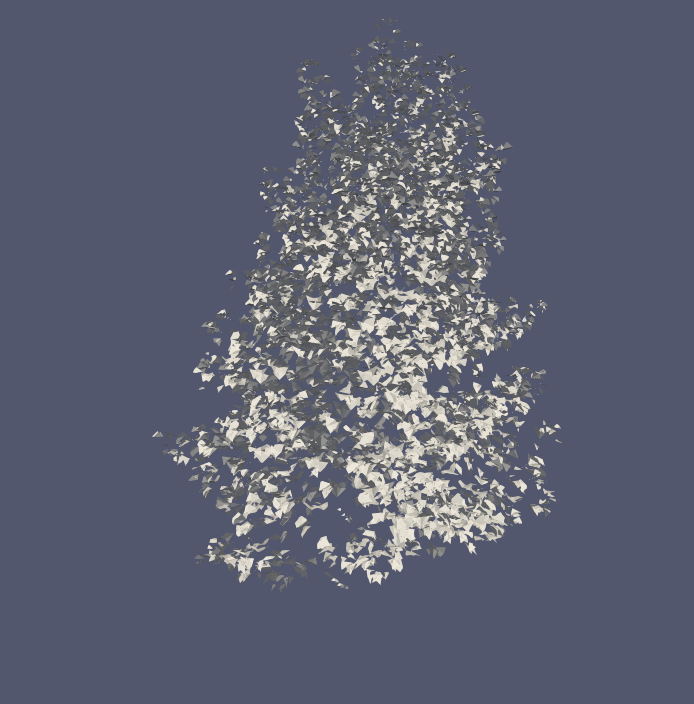
\includegraphics[width=1\textwidth]{images/tree-ginkgo.png}
        \captionsetup{font={scriptsize}}
        \caption{A cleaned Ginkgo (Oval tree)}
    \end{minipage}
    \begin{minipage}{0.30\textwidth}
        \centering
        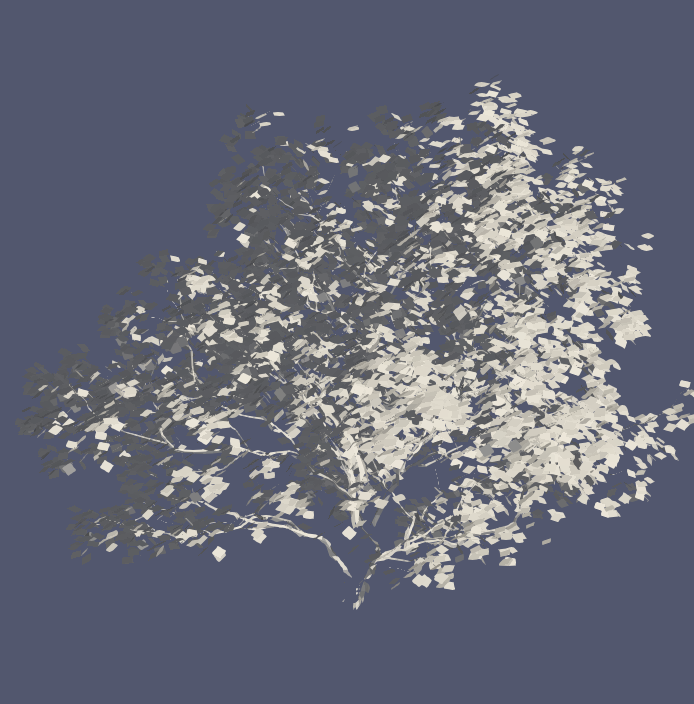
\includegraphics[width=1\textwidth]{images/tree-quercus.png}
        \captionsetup{font={scriptsize}}
        \caption{A cleaned Quercus (Round tree)}
    \end{minipage}
\end{figure}

Finally, using the CGAL 3D Alpha Wrapping algorithm (explained in \autoref{sec:alpha_wrapping}), 
we will generate reference tree
meshes for each shape at execution time. This pre-processing ensures
that the meshes are readily available in memory, eliminating the need to wrap and
write a \texttt{.stl} file each tree model individually during program execution.


The following images illustrate the results of the wrapping algorithm for different
\texttt{alpha} values (cf \autoref{sec:alpha_wrapping}) on our different tree models
 retrieve from \texttt{Sketchup}
(the trunk is separated from the foliage, each image is composed of two parts: 
the trunk and the foliage):


\begin{figure}[H]
    \centering
    \begin{minipage}{0.30\textwidth}
        \centering
        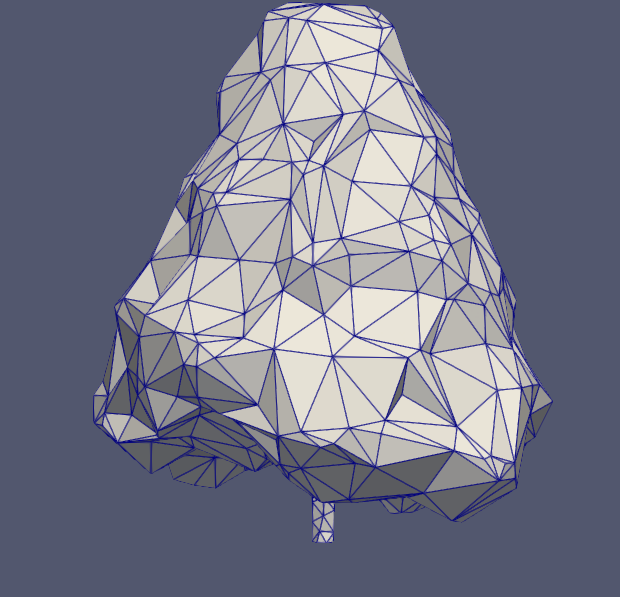
\includegraphics[width=1\textwidth]{images/tree-cone_lod1.png}
        \captionsetup{font={scriptsize}}
        \caption{Cone shaped lod1}
    \end{minipage}
    \begin{minipage}{0.30\textwidth}
        \centering
        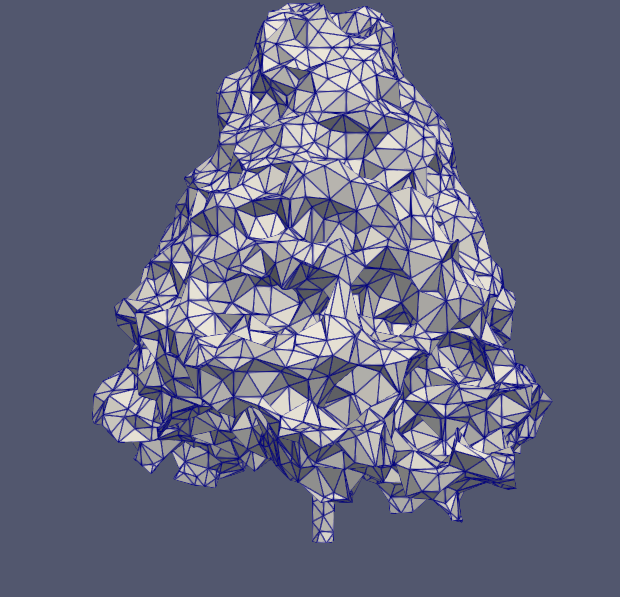
\includegraphics[width=1\textwidth]{images/tree-cone_lod2.png}
        \captionsetup{font={scriptsize}}
        \caption{Cone shaped lod2}
    \end{minipage}
    \begin{minipage}{0.30\textwidth}
        \centering
        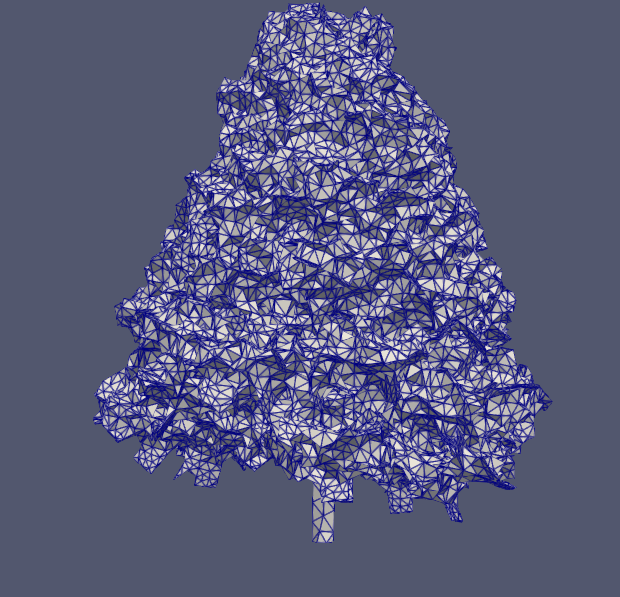
\includegraphics[width=1\textwidth]{images/tree-cone_lod3.png}
        \captionsetup{font={scriptsize}}
        \caption{Cone shaped lod3}
    \end{minipage}
\end{figure}

\begin{figure}[H]
    \centering
    \begin{minipage}{0.30\textwidth}
        \centering
        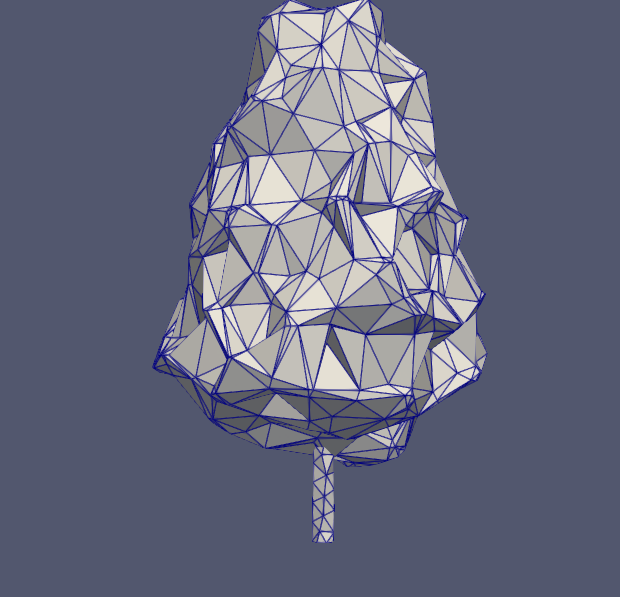
\includegraphics[width=1\textwidth]{images/tree-oval_lod1.png}
        \captionsetup{font={scriptsize}}
        \caption{Oval shaped lod1}
    \end{minipage}
    \begin{minipage}{0.30\textwidth}
        \centering
        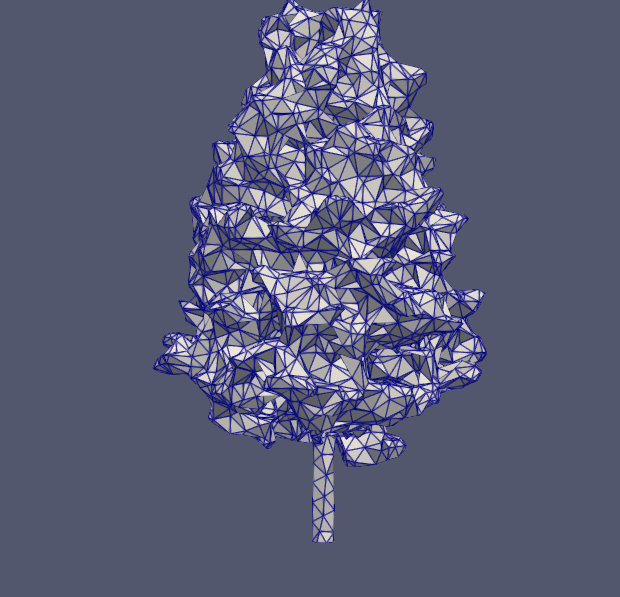
\includegraphics[width=1\textwidth]{images/tree-oval_lod2.png}
        \captionsetup{font={scriptsize}}
        \caption{Oval shaped lod2}
    \end{minipage}
    \begin{minipage}{0.30\textwidth}
        \centering
        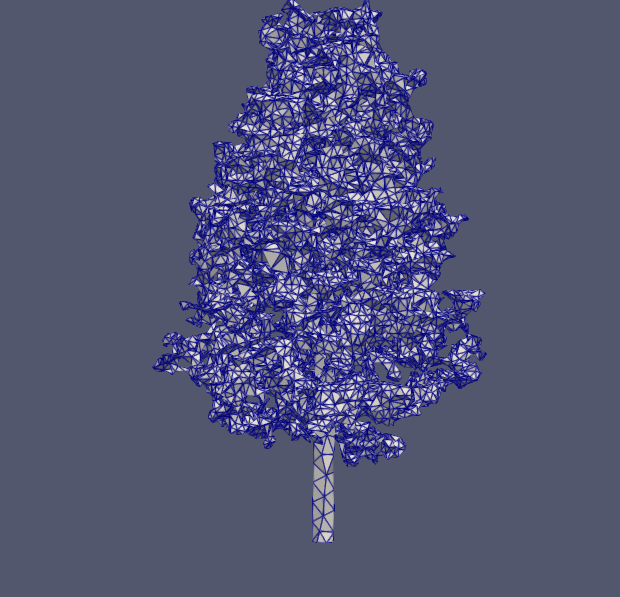
\includegraphics[width=1\textwidth]{images/tree-oval_lod3.png}
        \captionsetup{font={scriptsize}}
        \caption{Oval shaped lod3}
    \end{minipage}
\end{figure}

\begin{figure}[H]
    \centering
    \begin{minipage}{0.30\textwidth}
        \centering
        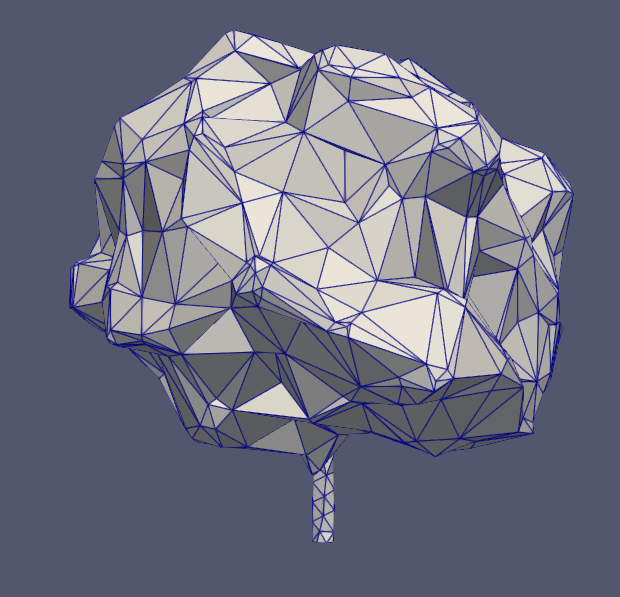
\includegraphics[width=1\textwidth]{images/tree-round_lod1.png}
        \captionsetup{font={scriptsize}}
        \caption{Round shaped lod1}
    \end{minipage}
    \begin{minipage}{0.30\textwidth}
        \centering
        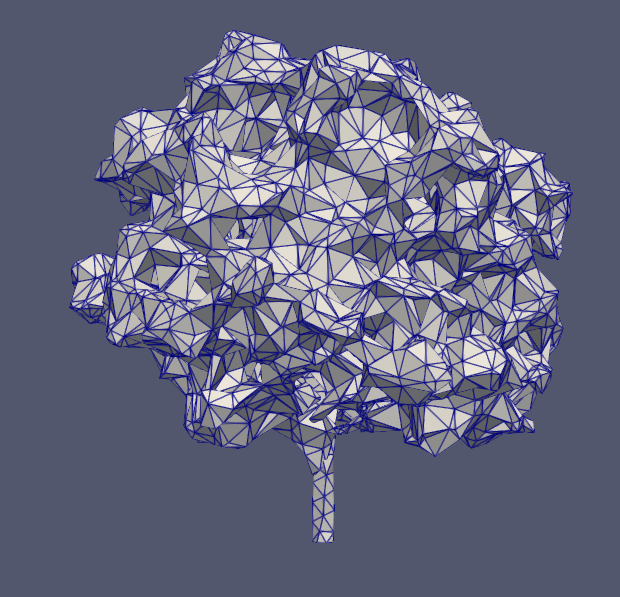
\includegraphics[width=1\textwidth]{images/tree-round_lod2.png}
        \captionsetup{font={scriptsize}}
        \caption{Round shaped lod2}
    \end{minipage}
    \begin{minipage}{0.30\textwidth}
        \centering
        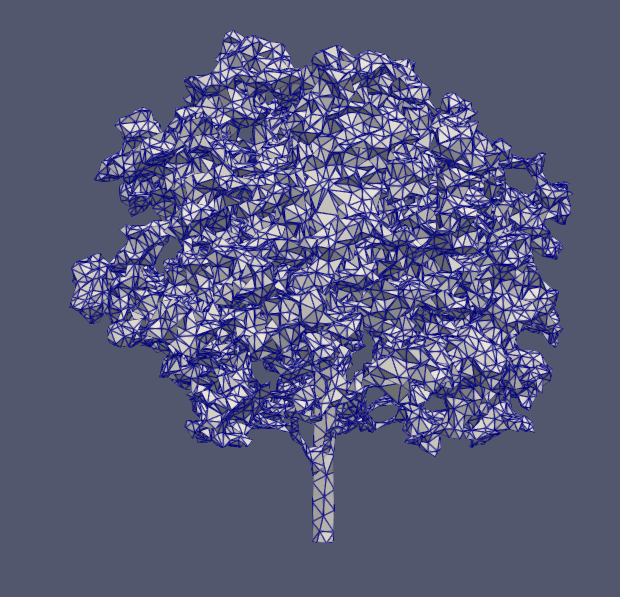
\includegraphics[width=1\textwidth]{images/tree-round_lod3.png}
        \captionsetup{font={scriptsize}}
        \caption{Round shaped lod3}
    \end{minipage}
\end{figure}


We used the following \texttt{alpha} values for each LOD:
\begin{table}[H]
    \centering
    \begin{tabular}{|l|c|c|c|c|}
    \hline
    Tree & LOD 0 & LOD 1 & LOD 2 & LOD 3 \\
    \hline
    Alpha & Nan & 20 & 50 & 100 \\
    \hline
    \end{tabular}
    \caption{Alpha values for each LOD}
    \label{tab:my_label}
\end{table}

(Reminder: LOD 0 is made with Gmsh not with the Alpha Wrapping algorithm.)

\subsubsection{Number of faces}
In simulation software, the number of faces in the mesh is crucial for
performance. The next table shows the relation between the LOD and the number of
 faces for each tree shape:

\begin{table}[H]
    \centering
    \begin{tabular}{|l|c|c|c|c|}
    \hline
    Tree & LOD 0 & LOD 1 & LOD 2 & LOD 3 \\
    \hline
    Trunk & 194 & 194 & 194 & 194 \\
    Cone & 874 & 894 & 6038 & 34260 \\
    Oval & 530 & 1260 & 9254 & 44942 \\
    Round & 1106 & 1198 & 10152 & 45164 \\
    \hline
    \end{tabular}
    \caption{Number of faces per tree shape type and LOD}
    \label{tab:my_label2}
\end{table}

\subsubsection{Leaf density}

As seasons change, trees undergo various stages of growth and leaf shedding.
To simulate these changes, we will implement different leaf densities for the
tree models. This will allow us to adjust the foliage's appearance and
complexity based on the time of year.\\

To achieve this we will iterate through the tree's faces of the foliage meshes 
and randomly label the faces with a \texttt{A, B, C, D} tag, each having a 
$25\%$ chance of being selected. This will allow us to represent the different
leaf densities; if all \texttt{A, B, C, D} tags are used, the tree will have
a full foliage, if only the tag \texttt{A} is used, the tree will have a low
foliage density, etc.\\

The following images depict the different leaf densities for the tree models:
...

The user will be able to specify which tags are applied in the \textit{config.json} 
file.

\subsubsection{Tree categorization}

To ensure the realism and accuracy of the tree models, we choose to categorize
them based on their shape. This categorization will help us
generate more realistic tree models and improve the overall quality of the
urban environment simulation. \\

The major issue will be to find a way to categorize the trees based on their shape
only knowing (at best) the genus, the species, the height, the circumference, and
the diameter of the crown. \\
If we had access to an image of the tree, we could use an image recognition
algorithm to categorize them based on their shape. \\
Another issue is that a young tree of a certain species will have a different 
shape than an old tree of the same species, and we don't have access to this information.
 The shape of a tree can also be influenced by its environment and the care it 
 receives (pruning, treatment, etc.). \\

 Hence, for the time being we will simply randomly assign a shape to the tree
 based on a uniform distribution. This will allow us to generate a variety of
 tree shapes and improve the realism of the urban environment simulation.
\subsection{Building mesh}

To test the integration of trees and buildings we will be working with is a 3D 
model of the Strasbourg city
center, provided in the \texttt{.stl} file format stored in the \texttt{data/terrain}
directory. This file contains the
geometric information of the terrain and buildings in the specified area,
which serves as the base for our project.

The \texttt{.stl}\cite{stl} (stereolithography) format is widely used for 3D printing
and computer-aided design (CAD). It represents the surface geometry of a 3D
object without any color, texture, or other attributes. The file comprises a
collection of triangular facets, each defined by its vertices and normal vector.

Here are some key details about the \texttt{.stl} file we are working with:
\begin{itemize}
    \item \textbf{File Name:} mesh\_lod1.stl
    \item \textbf{Region Covered:} Strasbourg city center
    \item \textbf{File Size:} 42,7 MB
    \item \textbf{Number of Vertices:} Approximately 120,959
    \item \textbf{Number of Facets:} Approximately 273,178
\end{itemize}

The 3D model includes various urban features such as buildings, streets, and
other infrastructure. This detailed representation is crucial for accurately
integrating tree models and conducting subsequent thermal and energy simulations.

Below are visual representations of the 3D model from different angles:

\begin{figure}[H]
    \centering
    \begin{minipage}{0.45\textwidth}
        \centering
        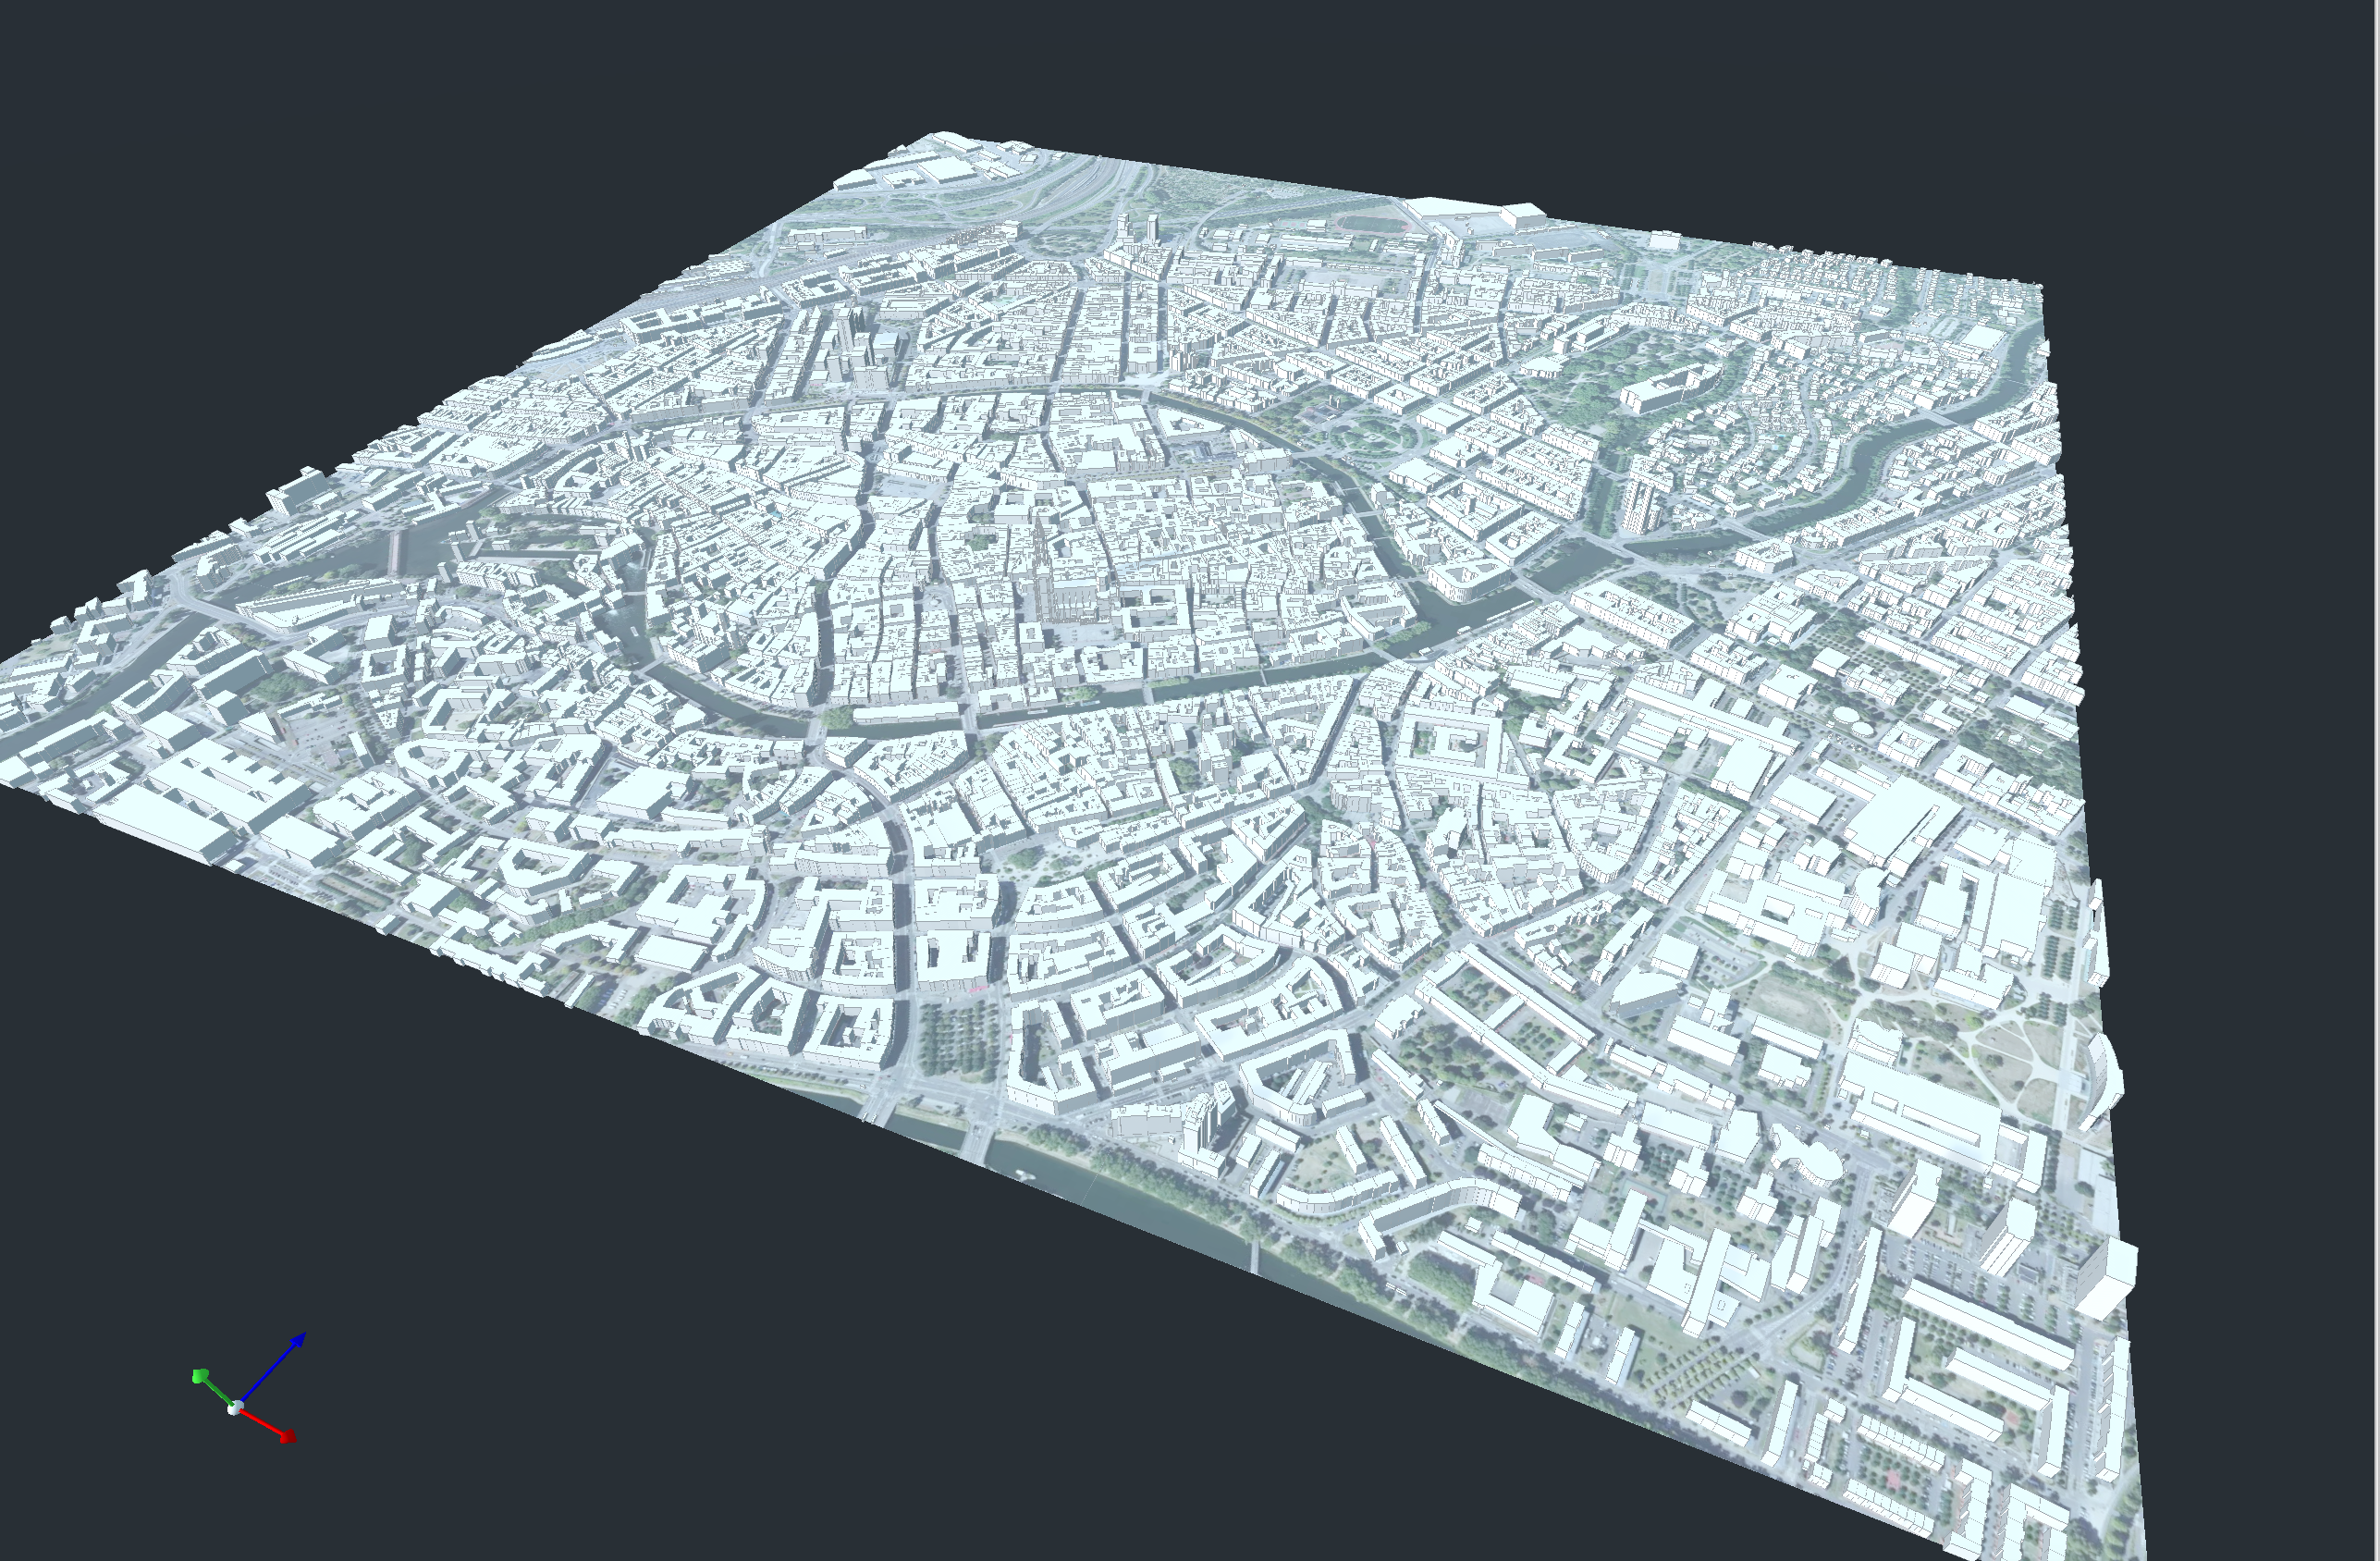
\includegraphics[width=1\textwidth]{images/strasbourg-mesh-1.png}
        \captionsetup{font={scriptsize}}
        \caption{Strasbourg 3D model (1)}
    \end{minipage}
    \begin{minipage}{0.45\textwidth}
        \centering
        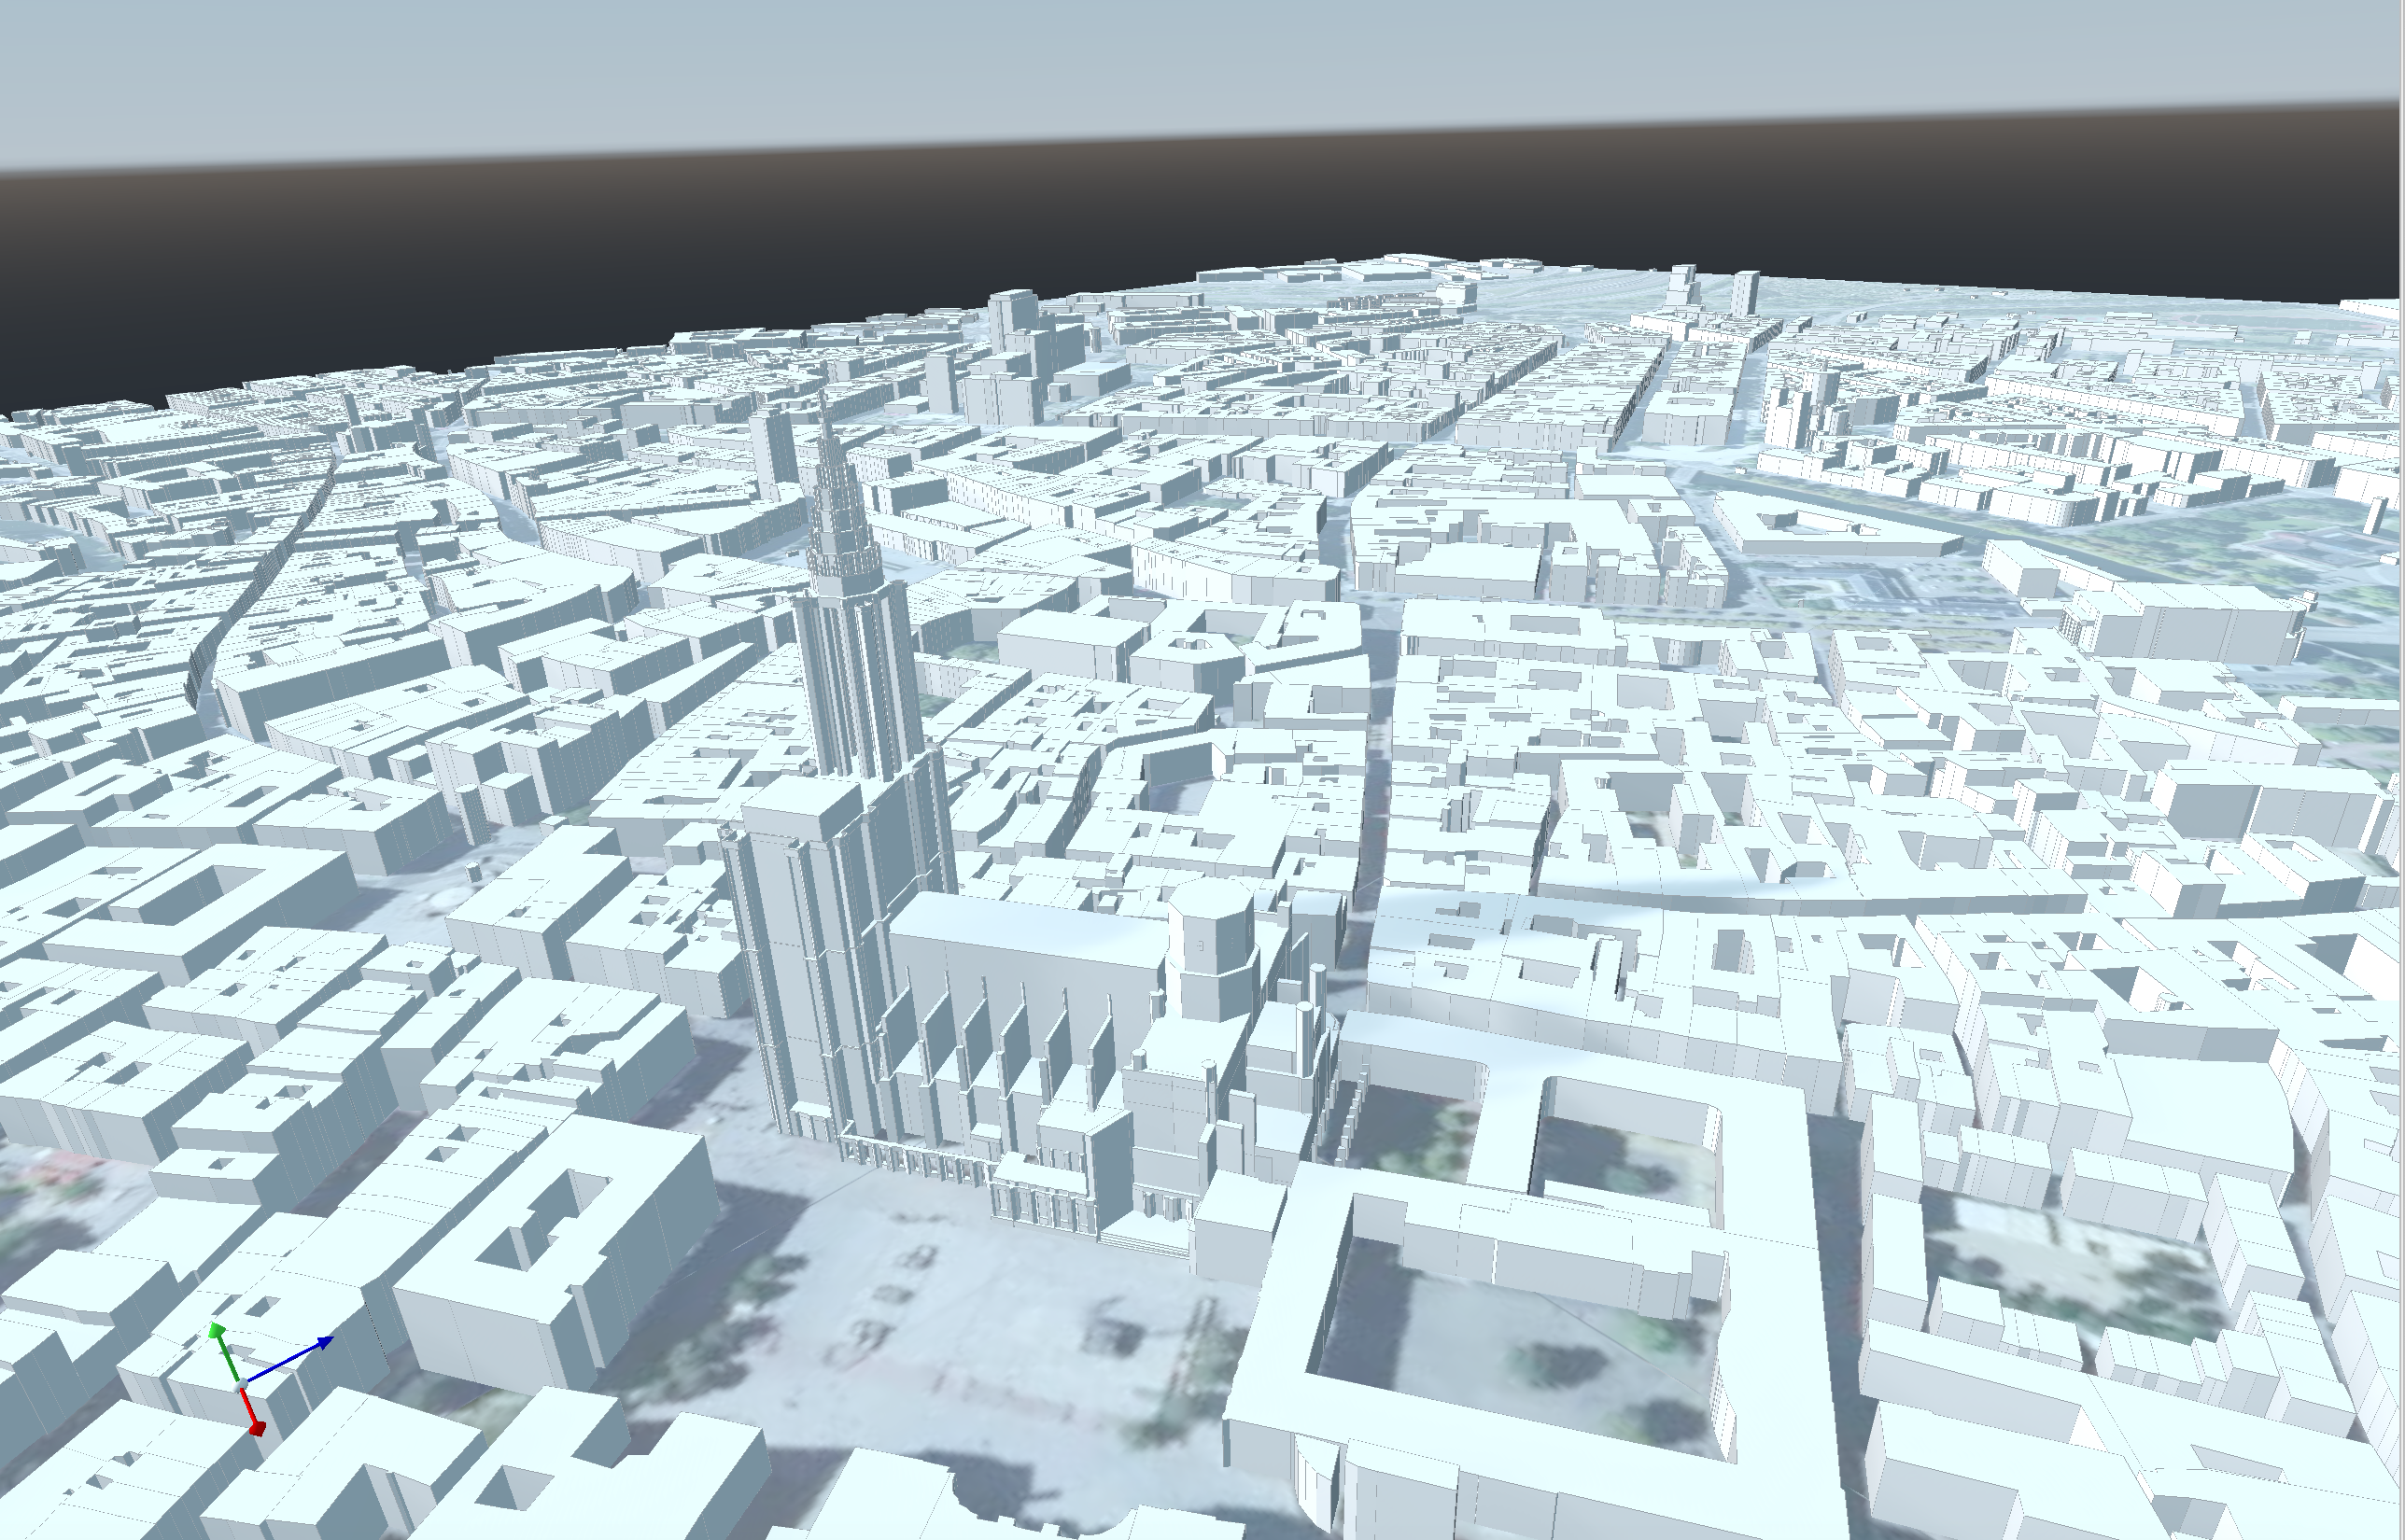
\includegraphics[width=1\textwidth]{images/strasbourg-mesh-2.png}
        \captionsetup{font={scriptsize}}
        \caption{Strasbourg 3D model (2)}
    \end{minipage}
\end{figure}

This dataset is instrumental in allowing us to accurately position tree models
within the urban landscape, ensuring that our simulations reflect realistic
interactions between vegetation and urban structures.


\subsection{Alpha Wrapping}
\label{sec:alpha_wrapping}
\begin{figure}[H]
    \centering
        \centering
        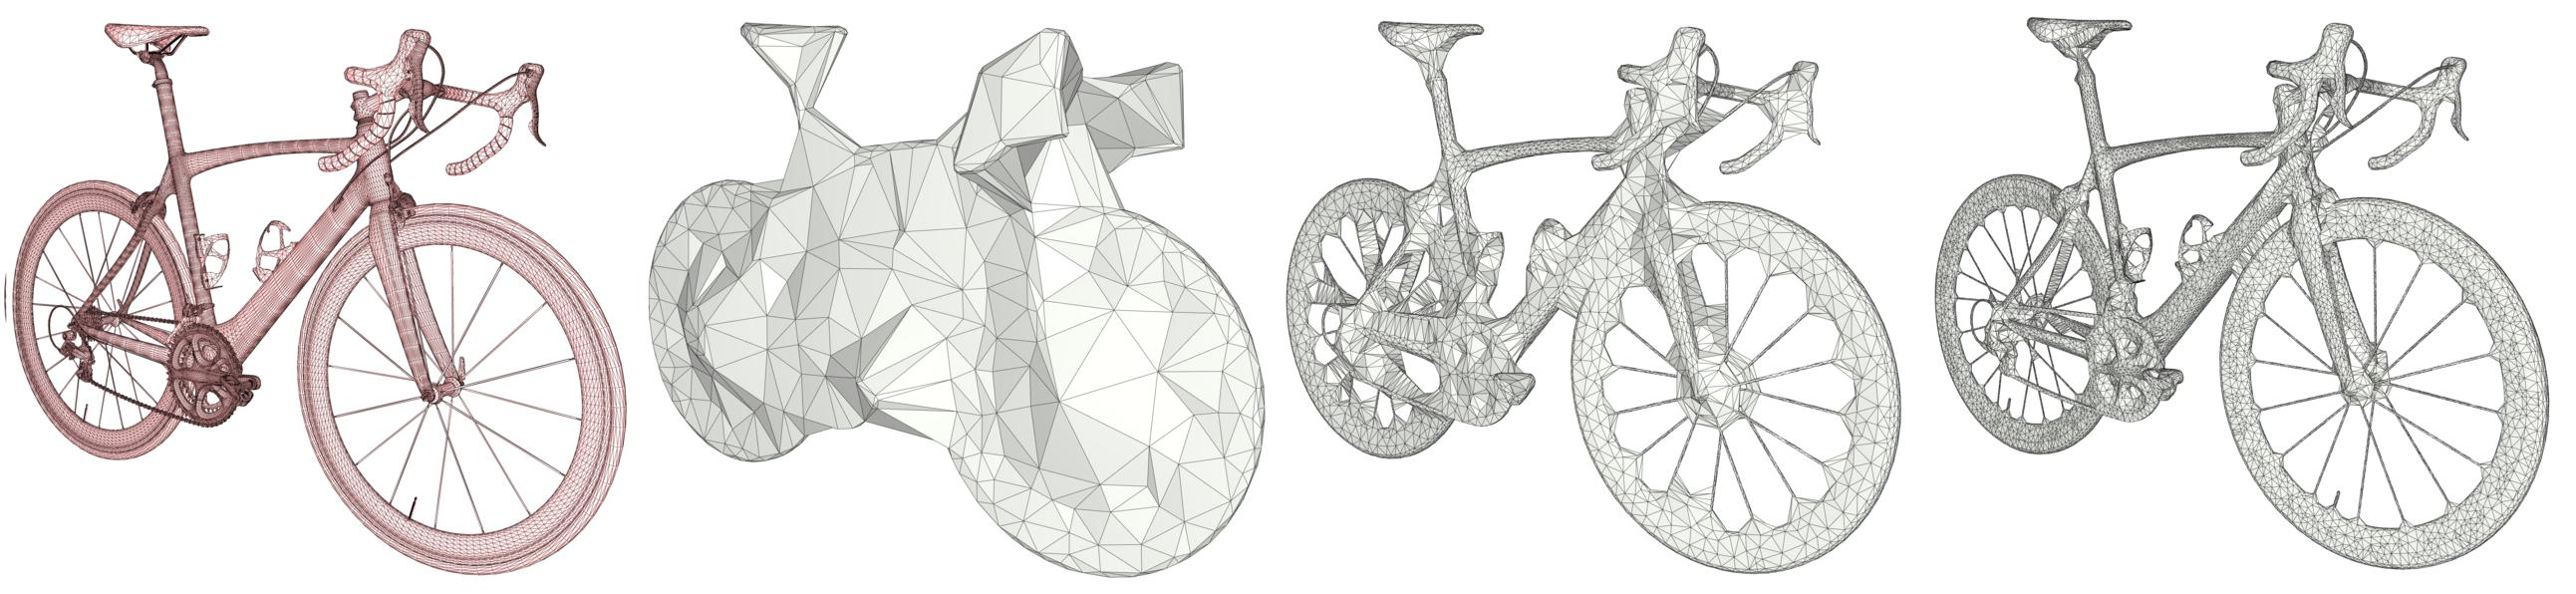
\includegraphics[width=\textwidth]{images/alpha-wrapping-bike.jpg}
        \captionsetup{font={scriptsize}}
        \caption{Different LOD of the Alpha Wrapping of a bike}
\end{figure}

\subsubsection{Approach}
To enclose a 3D model within a volume, various methods balance runtime and
approximation quality. Simple methods, like bounding boxes, have large errors.
Convex hulls improve quality but remain crude, especially for complex models.
Alpha shapes, a special case of the Delaunay triangulation, offer piecewise-linear
approximations but struggle with complex input data.

Inspired by alpha shapes, it uses shrink-wrapping, constructing a 3D Delaunay
triangulation and iteratively removing eligible boundary tetrahedra. This process
refines the triangulation, avoiding inner structures and unnecessary
computations. This method supports flexible input formats (triangle soups,
polygon soups, point clouds) and allows trading tightness for mesh complexity.

\subsubsection{Algorithm Initialization}
The algorithm starts by inserting the vertices of a bounding box into a 3D
Delaunay triangulation. In CGAL's 3D Delaunay triangulation, boundary facets
are adjacent to infinite cells tagged as outside, while finite tetrahedra are
tagged inside.

\subsubsection{Shrink-wrapping}
The algorithm traverses from outside to inside cells, using a priority queue of
Delaunay triangle facets (gates). A gate is alpha-traversable if its circumradius
exceeds a user-defined alpha. The priority queue, initialized with convex hull
gates, is sorted by decreasing circumradius. Traversal uses dual Voronoi edges.

When moving from an outside cell \( c_o \) to an inside cell \( c_i \) through
an alpha-traversable facet \( f \):

\begin{enumerate}
    \item Check for intersections between \( f \)'s dual Voronoi edge and
    the offset surface. Insert the first intersection point as a Steiner point
    into the triangulation.
    \item If no intersection but \( c_i \) intersects the input, project
    \( c_i \)'s circumcenter onto the offset surface and insert it as a Steiner point.
\end{enumerate}

Newly alpha-traversable gates are added to the queue. If neither criterion is
met, \( c_i \) is tagged outside, and its gates are pushed to the queue. The
process terminates when the queue empties, producing a triangle surface mesh from
 the Delaunay triangulation.

The figure below depicts the steps of the algorithm in 2D:
\begin{figure}[H]
    \centering
        \centering
        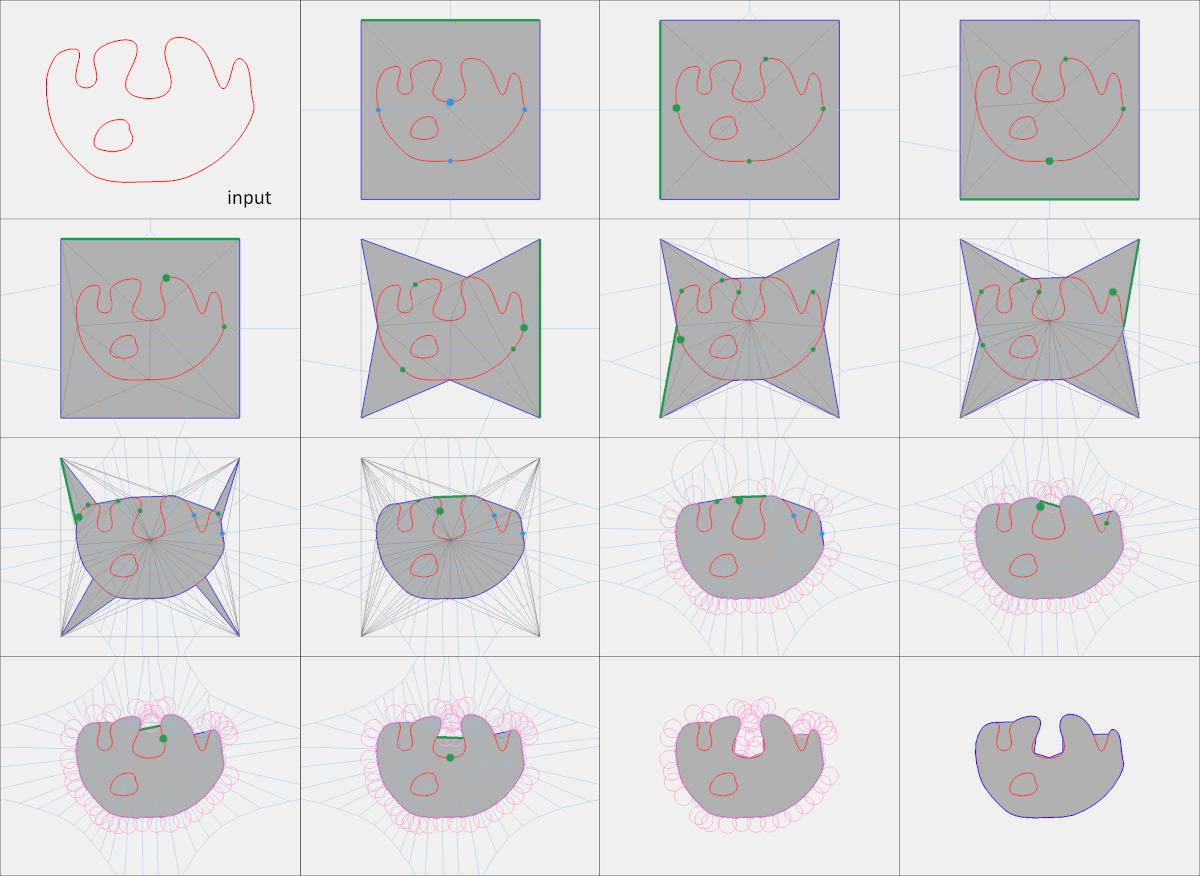
\includegraphics[width=\textwidth]{images/alpha-wrapping-steps.jpg}
        \captionsetup{font={scriptsize}}
        \caption{Steps of the shrink-wrapping algorithm in 2D. The algorithm
        initializes by inserting the bounding box corners into a Delaunay
        triangulation, tagging finite triangles inside. The current gate (green
        edge) is alpha-traversable. Adjacent triangles are tagged outside if
        they do not intersect the input. If they do, new Steiner points are
        inserted, and traversal resumes. The output edges (dark blue) separate
        inside from outside triangles.
        }
\end{figure}

\subsubsection{Termination and Guarantees}
The algorithm guarantees termination and produces a 2-manifold triangulated
surface mesh that encloses the input data. By wrapping from outside to inside
and refining the triangulation as needed, it ensures no intersecting cells are
flagged inside. Steiner points inserted during refinement break necessary cells,
 reducing circumradii and ensuring completion.

\subsection{Tree scaling}
In order to scale the trees to match the real world we will use the
following tree attributes retrieve from the \texttt{OpenStreetMap} data:
\begin{itemize}
    \item \texttt{height}: the height of the tree in meters.
    \item \texttt{diameter\_crown}: the diameter of the crown in meters.
    \item \texttt{circumference}: the circumference of the trunk in meters.
\end{itemize}

We will start by assuming those attributes exist and are correct.\\
Before scaling the tree we will add a random rotation to it to make the
simulation more realistic.\\
Then the next step will be to scale the tree to match the real world. To do this we
will scale the foliage and the trunk separately. The foliage will be scaled
using the \texttt{diameter\_crown} attribute and the trunk will be scaled using
the \texttt{circumference} attribute.\\

\begin{figure}[H]
    \centering
    \begin{minipage}{0.45\textwidth}
        \centering
        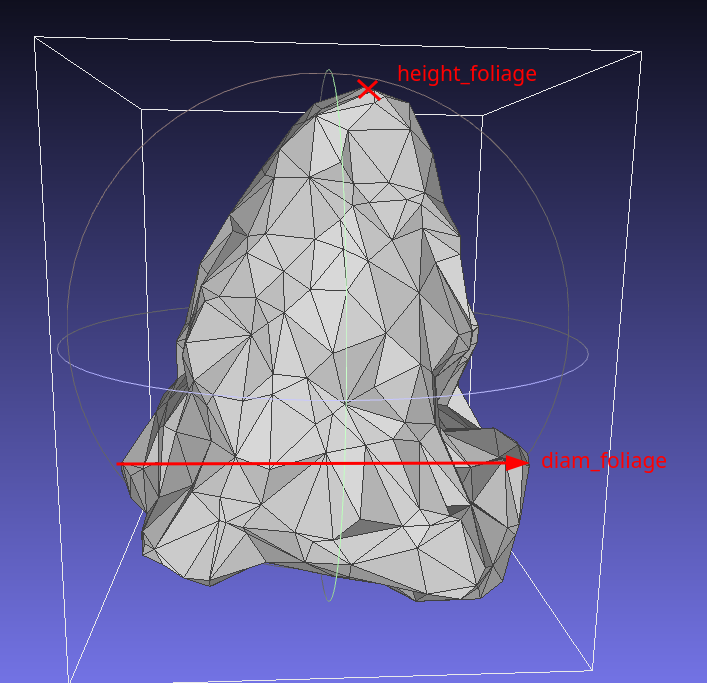
\includegraphics[height=7cm]{images/foliage_arrows.png}
        \captionsetup{font={scriptsize}}
        \caption{Foliage bounding box}
    \end{minipage}
    \begin{minipage}{0.45\textwidth}
        \centering
        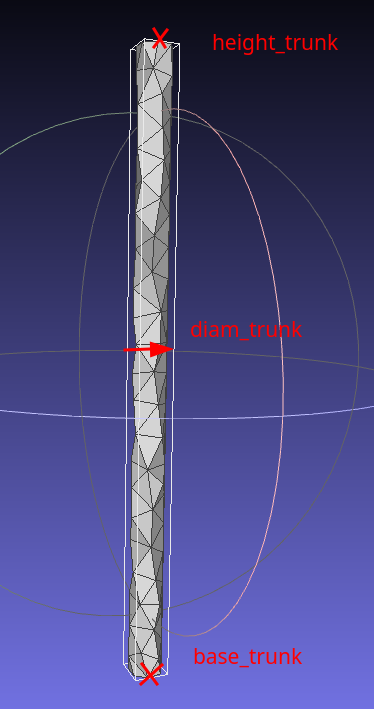
\includegraphics[height=7cm]{images/trunk_arrows.png}
        \captionsetup{font={scriptsize}}
        \caption{Trunk bounding box}
    \end{minipage}
\end{figure}

The \texttt{diameter\_crown} attribute depends on the shape of the tree as shown
in the next images:

\begin{figure}[H]
    \centering
    \begin{minipage}{0.45\textwidth}
        \centering
        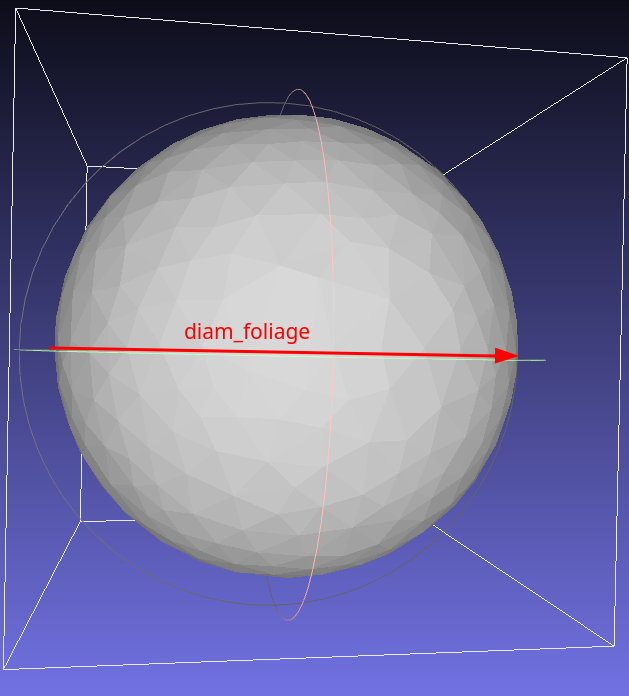
\includegraphics[height=7cm]{images/diam_foliage_round.png}
        \captionsetup{font={scriptsize}}
        \caption{Diameter crown round tree}
    \end{minipage}
    \begin{minipage}{0.45\textwidth}
        \centering
        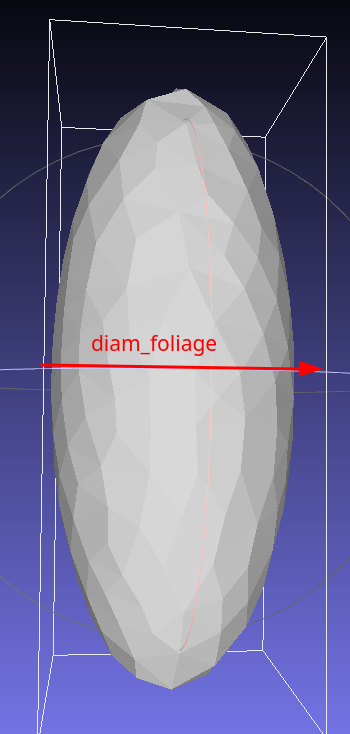
\includegraphics[height=7cm]{images/diam_foliage_oval.png}
        \captionsetup{font={scriptsize}}
        \caption{Diameter crown oval tree}
    \end{minipage}
\end{figure}

The \texttt{scaling factor} for the foliage will be calculated as follows:
\begin{equation}
    \text{scaling factor} = \frac{\text{diam\_foliage}}{\text{bbox.ymax()-bbox.ymin()}} + \text{noise}
\end{equation}

For the trunk it will be:
\begin{equation}
    \text{scaling factor} = \frac{\text{diam\_trunk}}{\text{bbox.ymax()-bbox.ymin()}} + \text{noise}  
\end{equation}

Where,
\begin{itemize}
    \item $\text{diam\_trunk} = \text{circumference} / \pi$
    \item $\text{bbox.ymax()-bbox.ymin()}$
    \item \texttt{noise} is a random value in the range 
    $[-\text{scaling factor} / 100, \text{scaling factor} / 100]$.
\end{itemize}

If the \texttt{circumference} (resp. \texttt{diameter\_crown}) is not available
we will use the \texttt{scaling factor} obtained from the other attribute to 
scale the tree.\\
If both attributes are missing we will use a default \texttt{height} value 
picked in a range defined by the user in the \textit{config.json} file.

\subsection{Tree placement}

Generated tree models will be integrated into terrain meshes to create comprehensive
3D urban models. To ensure precise integration into the terrain mesh (especially for large area), the tree models coordinates
(latitude, longitude) will be converted to Cartesian coordinates (x, y) using
a Mercator projection\cite{mercator-proj}.

\begin{figure}[H]
    \centering
    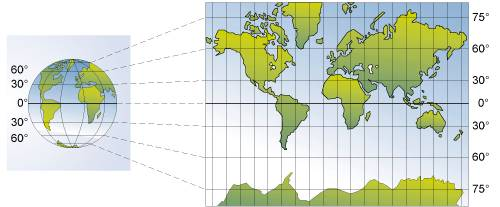
\includegraphics[width=1\textwidth]{images/mercator.jpg}
    \captionsetup{font={scriptsize}}
    \caption{Mercator's projection\cite{img:mercator}}
\end{figure}

This is the most common way to represent the Earth's surface on a plane and has
the advantage of being conformal, meaning that it preserves angles locally (hence
 its usage in sailings). \\
 In a Mercator projection, parallels and meridians are represented by straight
 orthogonal lines, with the equator being the horizontal line placed at the center
  of the map. The other parallels must necessarily be stretched (east-west
  stretching). This stretching is accompanied by a corresponding north-south
  stretching, so that the north-south scale is equal to the east-west scale
  everywhere. \\
  Mathematically, the Mercator projection is defined as follows: if a point on
  the sphere has a latitude $\phi$ and longitude $\lambda$ (with $\lambda_{0}$
  placed at the center of the map), then its projection on the Mercator map will
  have coordinates
  \begin{equation}
    \left\{
    \begin{array}{l}
        x =  \lambda - \lambda_{0} \\
        y =  \ln(\tan(\frac{\pi}{4} + \frac{\phi}{2}))
    \end{array}
    \right.
\end{equation}

To achieve this while taking into account that the Earth is not perfect sphere
we will assume the Earth is a geodesic defined as \texttt{WGS84}\cite{wgs84} and use
the \texttt{WGS84toCartesian}\cite{wgs84_to_cartesian} open source header-only
library to convert the coordinates.

The scaled foliage will be placed with the top of the bounding box at the
height of the tree. The trunk will be on the ground at the position of the tree.
To make sure the trunk is always at the right height we will use an abnormally
long trunk that will be cut to the right height. This will allow us to avoid having 
either the trunk floating in the air below the foliage or poking through it.

\begin{figure}[H]
    \centering
    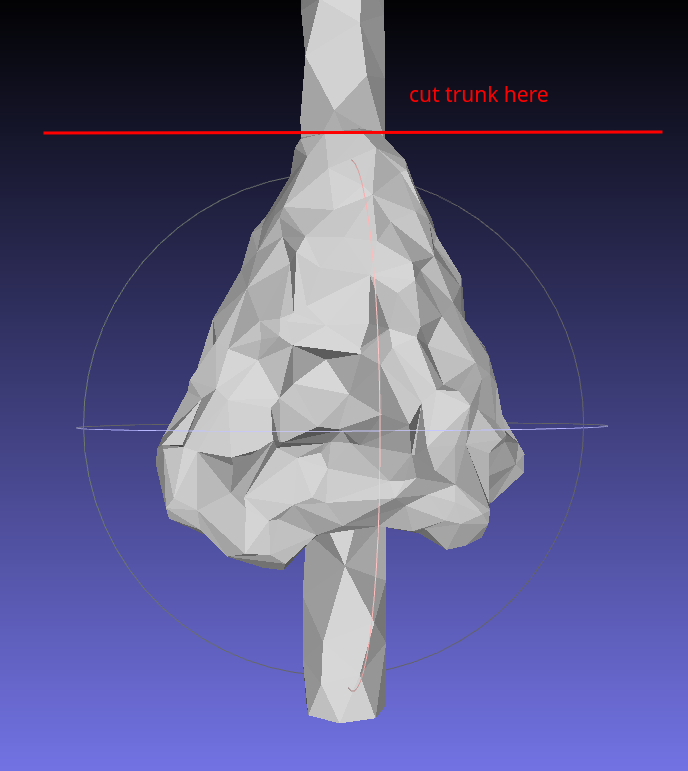
\includegraphics[height=7cm]{images/trunk_cut.png}
    \captionsetup{font={scriptsize}}
    \caption{Tree clipping}
\end{figure}

Then the union of all the tree meshed will need to be computed to create a single mesh
and avoid collision between the trees. \\
This will be achieved by considering all our meshes (trees, buildings, terrain) as
soup of triangle and  use the \texttt{autorefine\_triangle\_soup}\cite{auto-refine-triangle-soup}
function available in the master branch of the CGAL library. \\
Another approach could be to use the convex hull of the tree meshes, using the
intersection of the convex hulls to compute the union of the tree meshes.

\subsection{Metrics}
The complexity of the algorithms is a key metric to consider. \\
On each execution of the program, basics metrics will be exported to a text file in
the \texttt{output} directory. \\
These results will be analyzed more thoroughly in the \autoref{sec:Results}.

Example of the result's metrics for \textit{grande\_ile\_LOD1.txt}:

\begin{lstlisting}
Area: 561545 meters
Total number of trees: 409
Number of tree which had no height: 67
Number of faces: 482686
Time to mesh: 155.965 seconds, (2.59942 minutes)
\end{lstlisting}

\newpage

\section{Implementation}
\subsection{Doxygen documentation}

\texttt{Doxygen}\cite{doxygen} documentation is available for the project. Doxygen is a
documentation generator that produces comprehensive reference manuals from
annotated source code.

To generate the documentation, you can use the following command:

\begin{lstlisting}[language=bash]
doxygen Doxyfile
\end{lstlisting}

The documentation will be available in the \texttt{html} directory.\\
You can open it with the browser of your choice, for example with Firefox:

\begin{lstlisting}[language=bash]
firefox html/index.html
\end{lstlisting}

\newpage

\section{Results}
\label{sec:Results}
\subsection{Model integration}


\subsection{Complexity and performance analysis}

To assess the complexity and performance of our program, we executed it on
the High-Performance Computing (HPC) cluster Gaya. This cluster consists of a
DELL PowerEdge R7525 head node and six DELL PowerEdge R6525 compute nodes,
providing a total of 768 multi-threaded cores on the compute nodes and 96 cores
on the head node. Gaya offers 150 TB of storage for data and an extremely fast
15 TB NVME scratch space. The head node is equipped with two AMD EPYC 7552
48-Core Processors running at 2.2GHz, totaling 192 virtual cores, and 1024
GB of RAM. Each compute node features two AMD EPYC 7713 64-Core Processors
running at 2GHz, totaling 256 virtual cores, and 512 GB of RAM.
The nodes are interconnected via Broadcom Adv. Dual 10GBASE-T Ethernet and
Mellanox ConnectX-6 Dx Dual Port 100 GbE for MPI communication.\\
For our benchmarks, we used a single exclusive node with 256 cores and 512 GB
of RAM.


\section{Prospects}


\section{Conclusion}

\newpage

\section{References}
\bibliographystyle{unsrt}
\bibliography{references}

\end{document}